\section{Marco te\'orico y metodol\'ogico}
\label{sec:metodologia-marco-teorico}

\subsection{Elliott como punto de partida}
\label{subsec:elliott-punto-partida}

El punto de partida te\'orico del trabajo es la dificultad de convertir una
lectura discrecional y subjetiva del mercado en reglas que puedan calcularse y
revisarse de forma sistem\'atica. La teor\'ia de las Ondas de Elliott propone
interpretar los movimientos del precio mediante estructuras recurrentes de
impulso y correcci\'on \cite{frost_prechter_1985_elliott}. Estas estructuras se
entienden adem\'as como movimientos anidados, donde impulsos y retrocesos pueden
aparecer dentro de estructuras de mayor escala. Esta idea resulta atractiva para
un trabajo de trading algor\'itmico porque ofrece un lenguaje para hablar de
fases, retrocesos y continuaciones del precio. Sin embargo, tambi\'en plantea un
problema importante: el conteo de ondas puede depender del criterio del
analista, de la escala temporal utilizada y del punto exacto desde el que se
interpreta el movimiento.

En su formulaci\'on cl\'asica, Elliott suele representarse mediante un impulso
de cinco ondas en la direcci\'on principal del movimiento, seguido de una
correcci\'on en tres tramos etiquetados como A-B-C. Esta representaci\'on no
implica que el precio avance de forma ordenada ni que cada gr\'afico pueda
encajar siempre en el mismo patr\'on, pero ayuda a expresar una idea central:
los mercados alternan avances, retrocesos parciales y nuevas continuaciones.
La interpretaci\'on tradicional de esta teor\'ia tambi\'en incorpora una lectura
psicol\'ogica del mercado, donde las ondas se entienden como una forma de
representar cambios colectivos en expectativas, confianza, agotamiento o toma
de beneficios. En este TFG, esa dimensi\'on psicol\'ogica se utiliza solo como
marco conceptual y no como una variable medida directamente.

Para que este esquema pueda interpretarse como un conteo Elliott b\'asico no
basta con numerar m\'aximos y m\'inimos consecutivos. En un impulso est\'andar se
suelen exigir varias restricciones de validez: la onda 2 no debe retroceder por
debajo del origen de la onda 1. Adem\'as, la onda 3 no debe ser la m\'as corta
entre las ondas impulsivas 1, 3 y 5. Por \'ultimo, la onda 4 no deber\'ia solaparse
con el territorio de precio de la onda 1, salvo en estructuras especiales como diagonales. Estas
reglas no eliminan la subjetividad del conteo, pero ayudan a distinguir entre
una oscilaci\'on visual cualquiera y una hip\'otesis estructural que al menos
respeta las condiciones b\'asicas de la teor\'ia.

Por ese motivo, en esta memoria Elliott no se trata como una teor\'ia que deba
validarse de forma universal, sino como una referencia conceptual para estudiar
c\'omo se pueden formalizar ciertas lecturas del mercado. El inter\'es del TFG no
est\'a en afirmar que el precio siga siempre una estructura concreta, sino en
analizar qu\'e partes de esa lectura pueden transformarse en reglas, indicadores,
contextos y evidencias revisables. As\'i, una lectura t\'ecnica puede utilizarse
como punto de partida para el an\'alisis, pero no se convierte por s\'i sola en
una orden ni en una recomendaci\'on operativa.
La Figura~\ref{fig:elliott-5-abc-esquema} muestra de forma esquem\'atica la
estructura b\'asica que sirve como referencia conceptual.

\begin{figure}[!htbp]
\centering
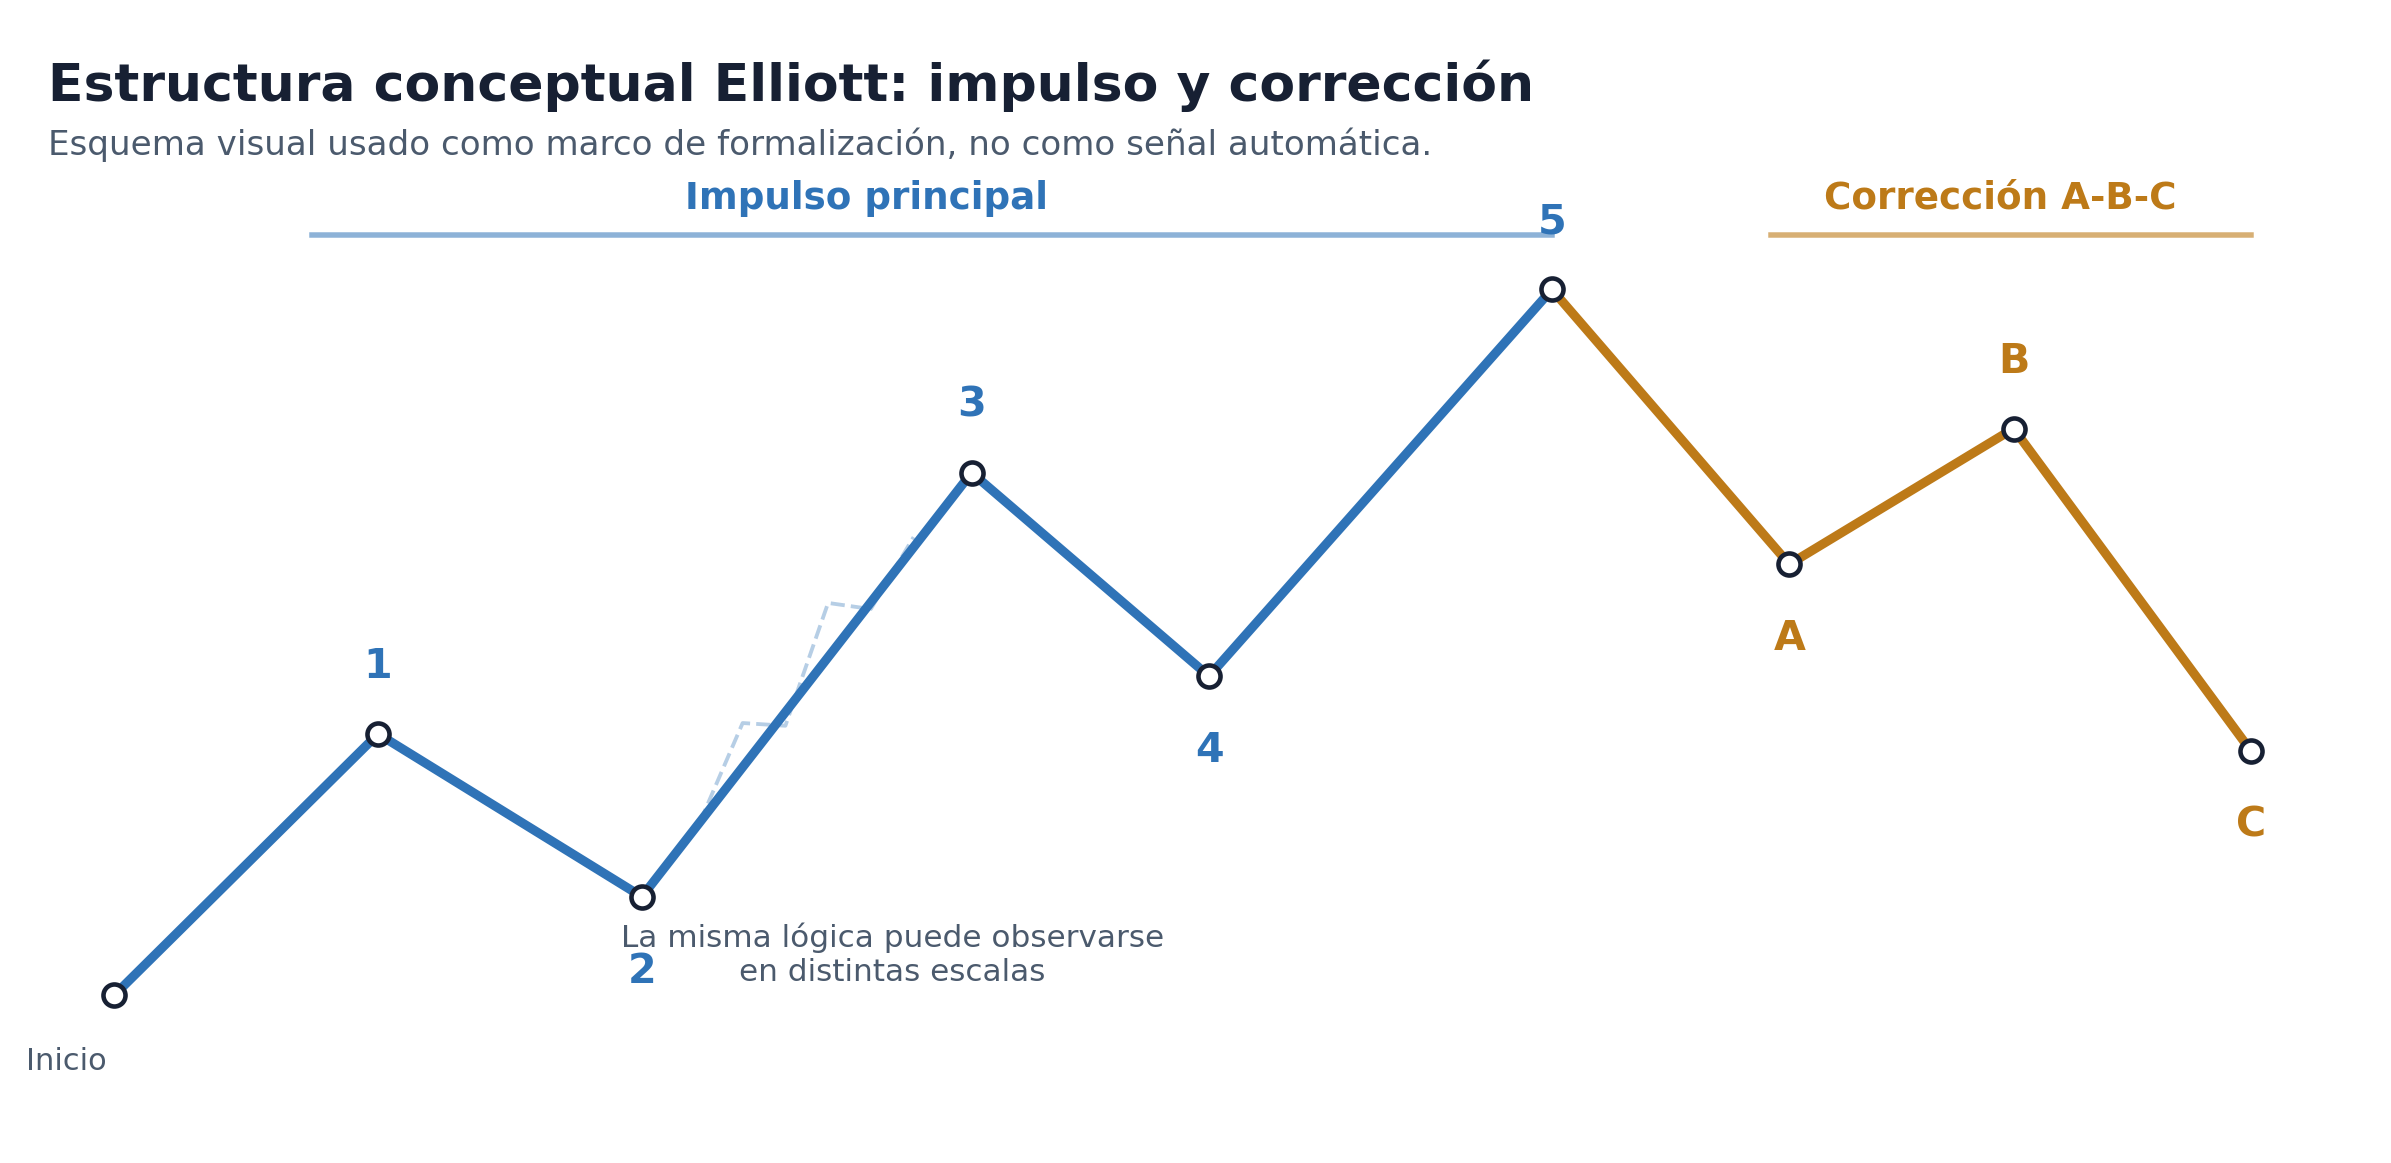
\includegraphics[width=0.95\textwidth]{figs/canonicas/metodologia/elliott_5_abc_esquema_canonico.png}
\caption[Esquema conceptual Elliott 5 + ABC]{Esquema conceptual de una estructura Elliott de impulso y correcci\'on.
La figura representa cinco ondas en la direcci\'on principal y una correcci\'on
A-B-C posterior; no constituye una regla autom\'atica de entrada ni una garant\'ia
de comportamiento del precio.}
\label{fig:elliott-5-abc-esquema}
\end{figure}

\subsection{Men\'endez Larre como referencia de formalizaci\'on}
\label{subsec:menendez-referencia-formalizacion}

Dentro de ese marco, el enfoque de Men\'endez Larre se utiliza como una
referencia metodol\'ogica para aproximar la teor\'ia de Elliott a un conjunto de
criterios m\'as mecanizables \cite{menendez_larre_2016_ondas}. Su planteamiento
relaciona la lectura de ondas con fractalidad, Fibonacci, indicadores y trabajo
en varios marcos temporales. Para este TFG, esa aportaci\'on resulta \'util no
porque resuelva por s\'i sola la subjetividad del conteo, sino porque ofrece una
forma concreta de pensar la transici\'on entre an\'alisis visual y reglas
programables.

La memoria toma esta referencia con un alcance acotado. El enfoque de Men\'endez
se emplea como apoyo para transformar una lectura visual de ondas en criterios
m\'as concretos y revisables. En el desarrollo del TFG, esa formalizaci\'on se
organiza mediante la separaci\'on entre la detecci\'on de posibles setups, la
informaci\'on de contexto, las se\~nales usadas para estudio y cualquier paso
relacionado con una ejecuci\'on operativa. La formalizaci\'on concreta de sus
reglas y el backtesting realizado se tratan m\'as adelante como una l\'inea
experimental propia, separada del benchmark principal del trabajo. Por tanto,
no se presenta como una garant\'ia de robustez ni como una estrategia final
cerrada.

\subsection{Fractalidad y lectura multiescala}
\label{subsec:fractalidad-multiescala}

La idea de fractalidad aparece en el trabajo como una motivaci\'on para estudiar
el mercado en distintas escalas temporales. En finanzas, la literatura sobre
precios especulativos y mercados fractales ha se\~nalado que las series de
precios pueden mostrar comportamientos complejos, colas pesadas, dependencia de
escala y estructuras que no siempre encajan bien con modelos simples
\cite{mandelbrot_1963_speculative_prices,
mandelbrot_hudson_2004_misbehavior,peters_1994_fractal_market}. En este TFG,
esa perspectiva se utiliza de forma prudente: sirve para justificar por qu\'e se
observan marcos temporales diferentes y por qu\'e una se\~nal aislada puede necesitar
contexto, pero no para afirmar que exista una pauta explotable de forma
autom\'atica.

Esta lectura multiescala tambi\'en ayuda a explicar la separaci\'on entre
estrategias, contexto y herramientas de revisi\'on. Una regla puede identificar una
condici\'on concreta en un marco temporal, mientras que otros elementos pueden
aportar informaci\'on sobre tendencia, volatilidad, pivotes, retrocesos o
estructura. La metodolog\'ia del TFG se apoya en esa separaci\'on para evitar que
todo se reduzca a una se\~nal de entrada. Tambi\'en permite mantener visible qu\'e
parte del sistema calcula una condici\'on, qu\'e parte aporta contexto y qu\'e parte
queda reservada a la revisi\'on humana.

\subsection{Consecuencia metodol\'ogica para el TFG}
\label{subsec:consecuencia-metodologica}

A partir de este marco, el trabajo adopta una decisi\'on metodol\'ogica clara:
las ideas procedentes del an\'alisis t\'ecnico no se incorporan como reglas
operativas directas, sino como hip\'otesis de formalizaci\'on. Cada regla debe
poder traducirse a condiciones calculables, evaluarse sobre datos hist\'oricos,
compararse con estrategias de referencia y conservar evidencias que permitan
revisar qu\'e se ha hecho. De este modo, la memoria no depende de una lectura
subjetiva de un gr\'afico, sino de un flujo en el que los datos, las reglas, las
pruebas y las salidas quedan conectados.

Esta decisi\'on tambi\'en condiciona el dise\~no del sistema. El Screener se
concibe como un m\'odulo de filtrado y priorizaci\'on de setups. La lectura
estructural del precio se incorpora como una capa de contexto. AI Analyst act\'ua
como asistente de an\'alisis sin capacidad de aprobar operaciones.
MT5 se integra en varias capas diferenciadas: lectura de datos, consulta de
estado para observabilidad, generaci\'on de propuestas de orden y env\'io
controlado de \'ordenes desde el bot. En conjunto, estos elementos permiten
pasar de una lectura t\'ecnica del mercado a un flujo revisable, donde la
detecci\'on, la evaluaci\'on, la supervisi\'on y la posible ejecuci\'on quedan
separadas.

\section{Datos del estudio e ingesta}
\label{sec:datos-ingesta}

\subsection{Origen y granularidad de los datos}
\label{subsec:origen-granularidad-datos}

La base cuantitativa del trabajo est\'a formada por series de precios de
mercado en formato OHLC: apertura, m\'aximo, m\'inimo y cierre de cada vela.
Estas series se complementan con campos auxiliares disponibles en la fuente,
como volumen, \textit{spread} o diferencia entre precios de compra y venta.
Tambi\'en se registran s\'imbolo, grupo de mercado y timeframe. El uso de
datos agregados por vela permite estudiar reglas de entrada, salida, contexto
y revisi\'on. As\'i se evita depender de informaci\'on intrabar que no est\'a
disponible de forma homog\'enea en todos los bloques del proyecto.

Los datos de mercado se obtienen a trav\'es de la integraci\'on de MetaTrader 5
con Python y se almacenan en una base de datos local para su reutilizaci\'on
posterior \cite{metatrader5_python_docs}. El estudio trabaja principalmente con
activos de divisas, metales e \'indices, y utiliza distintos timeframes,
entendidos como marcos temporales de agregaci\'on de las velas, intradiarios y
diarios como M15, M30, H1, H4 y D1.
No todos los bloques usan siempre la misma
combinaci\'on: las estrategias, los benchmarks, el estudio Men\'endez y el
Trading Center seleccionan los timeframes necesarios para su propio objetivo
experimental.
En esta notaci\'on, M15 y M30 representan velas de 15 y 30 minutos; H1 y H4,
velas de una y cuatro horas; y D1, velas diarias.

El preprocesamiento de las series, la construcci\'on de tablas y la generaci\'on
de figuras se realizan mediante scripts locales del proyecto. En esta parte se
prioriza documentar la procedencia de los datos, la configuraci\'on de las
pruebas y las salidas generadas, antes que citar cada librer\'ia auxiliar
empleada para tareas de c\'alculo o visualizaci\'on.

Desde el punto de vista de Ciencia de Datos, cada vela puede entenderse como
una observaci\'on temporal agregada. La Tabla \ref{tab:estructura-datos-ohlc}
resume la estructura b\'asica que se utiliza de forma recurrente en la memoria.
No todas las salidas intermedias contienen exactamente las mismas columnas,
pero esta organizaci\'on permite situar los campos principales que alimentan
ingesta, backtesting, Screener y dashboard.

\begin{table}[H]
\centering
\small
\begin{tabular}{p{0.22\textwidth} p{0.34\textwidth} p{0.34\textwidth}}
\hline
\textbf{Campo} & \textbf{Significado} & \textbf{Uso dentro del TFG} \\
\hline
\texttt{timestamp} & Fecha y hora de cierre de la vela. & Orden temporal, control de vela cerrada y sincronizaci\'on entre timeframes. \\
\texttt{symbol} & Activo analizado. & Agrupaci\'on por divisas, metales o \'indices, y revisi\'on individual en dashboard. \\
\texttt{timeframe} & Granularidad de la serie, por ejemplo M30, H1, H4 o D1. & Define el timeframe operativo y el timeframe de contexto de cada prueba. \\
\texttt{OHLC} & Apertura, m\'aximo, m\'inimo y cierre de la vela; campos \texttt{open}, \texttt{high}, \texttt{low} y \texttt{close}. & Base para reglas de entrada, rupturas, niveles Fibonacci, stops y objetivos. \\
\texttt{volume}/\texttt{spread} & Campos auxiliares disponibles; el \textit{spread} aproxima la diferencia entre precio de compra y venta. & Apoyo para caracterizar condiciones de mercado y costes de simulaci\'on cuando procede. \\
Metadatos de extracci\'on & Fuente, cobertura, fecha de actualizaci\'on y comprobaciones de calidad. & Trazabilidad, detecci\'on de datos desactualizados y reproducci\'on de resultados. \\
\hline
\end{tabular}
\caption[Estructura conceptual de datos OHLC]{Estructura conceptual de los datos de mercado usados en el TFG. La unidad
b\'asica es una vela OHLC cerrada, complementada con campos auxiliares y
metadatos de extracci\'on.}
\label{tab:estructura-datos-ohlc}
\end{table}

La Tabla~\ref{tab:ejemplo-cobertura-datos} muestra un ejemplo real de cobertura
registrada en una auditor\'ia de datos. No representa un resultado de estrategia,
sino la forma en la que el sistema conserva informaci\'on sobre disponibilidad
temporal, granularidad y n\'umero de observaciones antes de alimentar backtests o
vistas de revisi\'on. Debajo se incluyen tres filas reales extra\'idas de un
archivo local \texttt{ohlc\_window.csv}, para mostrar c\'omo se organiza una
observaci\'on de mercado antes de ser usada por las reglas.

\begin{table}[H]
\centering
\scriptsize
\begin{tabular}{llllr}
\hline
\textbf{Activo} & \textbf{Grupo} & \textbf{Timeframe} & \textbf{Cobertura temporal} & \textbf{Velas} \\
\hline
\texttt{AUDCAD.r} & Divisas principales & M15 & 2022-01-19 03:00--2026-03-17 10:00 & 103306 \\
\texttt{AUDCAD.r} & Divisas principales & H1 & 2021-05-26 00:00--2026-03-17 09:00 & 29913 \\
\texttt{AUDCAD.r} & Divisas principales & H4 & 2021-05-26 00:00--2026-03-17 04:00 & 7479 \\
\hline
\end{tabular}

\vspace{0.7em}

\begin{tabular}{lllrrrr}
\hline
\textbf{Cierre vela} & \textbf{Activo} & \textbf{Timeframe} & \textbf{Open} & \textbf{High} & \textbf{Low} & \textbf{Close} \\
\hline
2026-04-16 04:00 & \texttt{CADCHF.r} & H4 & 0.56897 & 0.56929 & 0.56873 & 0.56921 \\
2026-04-16 08:00 & \texttt{CADCHF.r} & H4 & 0.56921 & 0.57046 & 0.56908 & 0.56996 \\
2026-04-16 12:00 & \texttt{CADCHF.r} & H4 & 0.56996 & 0.57111 & 0.56992 & 0.57099 \\
\hline
\end{tabular}
\caption[Ejemplo de cobertura y filas OHLC]{Ejemplo de cobertura auditada y formato tabular de filas OHLC.
La parte superior resume disponibilidad temporal; la parte inferior muestra
filas reales de una ventana OHLC H4 conservada en un archivo local del
proyecto. Cada vela queda identificada por timestamp, activo y timeframe.}
\label{tab:ejemplo-cobertura-datos}
\end{table}

La Tabla~\ref{tab:dimensiones-datos-estudio} resume las dimensiones principales
de los datos utilizados en los bloques m\'as relevantes del trabajo. La tabla
muestra de forma compacta qu\'e tipo de informaci\'on alimenta cada parte del
sistema y evita mezclar series de mercado, bloques de backtesting, cortes del
dashboard y auditor\'ias t\'ecnicas.

\begin{table}[H]
\centering
\scriptsize
\begin{tabular}{@{}p{0.21\textwidth} p{0.23\textwidth} p{0.16\textwidth} p{0.30\textwidth}@{}}
\hline
\textbf{Bloque} & \textbf{Activos o grupos} & \textbf{Timeframes} & \textbf{Dimensi\'on usada en la memoria} \\
\hline
Ingesta y dashboard & Divisas, metales e \'indices & M15, M30, H1, H4 y D1 & Series OHLC cerradas con metadatos de cobertura, actualizaci\'on y fuente. \\
Benchmark principal & Tres grupos de activos & M30:H1, H1:H4 y H4:D1 & Nueve bloques independientes por regla, con operaciones y m\'etricas agregadas por bloque. \\
L\'inea Men\'endez/Elliott & Divisas principales & M30:H4 & Validaci\'on acotada de variantes metodol\'ogicas y registros de operaciones por variante. \\
WaveCount/\\WeaveCount & Divisas, metales e \'indices & H1 y H4 & Noventa y cuatro combinaciones s\'imbolo/timeframe: 47 en H1 y 47 en H4. \\
Screener y revisi\'on & Corte publicado en \texttt{latest} & Timeframes usados por cada setup & Corte final con 97 candidatos revisables: 90 \texttt{macd\_breakout}, 4 \texttt{fib\_limit} y 3 \texttt{rsi\_trend\_reversal}. \\
\hline
\end{tabular}
\caption[Dimensiones principales de los datos del estudio]{Dimensiones principales de los datos empleados en los bloques del TFG. La tabla ayuda a distinguir entre series de mercado, bloques de backtesting, validaciones estructurales y cortes de revisi\'on del dashboard.}
\label{tab:dimensiones-datos-estudio}
\end{table}

El calendario econ\'omico y el contexto macroecon\'omico no se
incorporan como una tabla estructurada dentro del conjunto principal de datos.
Durante el desarrollo se valor\'o esta posibilidad, pero su obtenci\'on estable
presentaba limitaciones pr\'acticas: algunas interfaces de programaci\'on (API)
tienen coste y varias fuentes web no permiten una extracci\'on automatizada
sencilla para un uso acad\'emico.
Por ese motivo, ese material queda separado de las series OHLC y se consulta
solo cuando resulta necesaria para un informe del AI Analyst. En ese caso, el
analista consulta fuentes oficiales o institucionales seg\'un el activo
revisado, sin convertir esa consulta en una base de datos macroecon\'omica
propia del proyecto.

\subsection{Ingesta incremental y actualizaci\'on}
\label{subsec:ingesta-incremental}

La ingesta se dise\~na para actualizar los datos de forma incremental. Cuando
existen registros previos de un s\'imbolo y timeframe, el proceso recupera la
fecha m\'as reciente almacenada. A partir de ese punto, solicita a MT5 solo el
tramo necesario, manteniendo un peque\~no solapamiento temporal para evitar
gaps o huecos temporales en el enlace entre actualizaciones. Si no existen datos previos, se realiza una
carga hist\'orica inicial. Esta organizaci\'on reduce trabajo repetido y permite
mantener una base local utilizable para backtesting, Screener y revisi\'on.

El sistema tambi\'en incorpora un scheduler as\'incrono por cadencias. La
actualizaci\'on de M15, M30 y los timeframes superiores se organiza mediante
bucles independientes alineados con los cierres esperados de cada ventana de
datos. Esta parte requiri\'o tratar con cuidado la diferencia entre la zona
horaria local y la hora del servidor del broker. En timeframes como H4 o
D1, un desfase puede hacer que una vela se lea demasiado pronto o con retraso.
Por tanto, el objetivo no es registrar cada variaci\'on del precio, sino
actualizar la base cuando se dispone de nuevas velas cerradas. Esta decisi\'on es
coherente con el uso posterior de los datos en backtests y herramientas de
revisi\'on, donde una se\~nal solo debe evaluarse con informaci\'on ya disponible.

Tras la ingesta, el Trading Center puede activar una capa de actualizaci\'on que
consume los datos preparados y actualiza los archivos de evidencia necesarios
para la interfaz. Esta capa no sustituye al
scheduler de datos: act\'ua por encima, validando que la informaci\'on necesaria
est\'a disponible antes de promover una nueva versi\'on de los archivos de consulta.

\subsection{Control de calidad y prevenci\'on de informaci\'on futura}
\label{subsec:control-calidad-datos}

Un aspecto central del tratamiento de datos es trabajar con velas cerradas. El
proceso de ingesta filtra la vela abierta utilizando la hora de servidor de MT5
cuando est\'a disponible. Este filtro se aplica tanto en la actualizaci\'on
incremental como en la carga hist\'orica. Su objetivo es evitar que una
estrategia utilice precios de una vela que todav\'ia no habr\'ia estado cerrada
en el momento de decisi\'on. Esta precauci\'on se relaciona directamente con la
prevenci\'on de \textit{look-ahead} en las pruebas hist\'oricas.

Sobre la base local se han incorporado comprobaciones de calidad orientadas a
detectar problemas frecuentes en series financieras: duplicados por
s\'imbolo/timeframe, valores OHLC inv\'alidos, nulos relevantes, timestamps no
alineados, gaps o huecos temporales y datos desactualizados. Estas comprobaciones no solo revisan si
la estructura de los datos es correcta, sino tambi\'en si la \'ultima vela
disponible es suficientemente reciente para el uso previsto. De esta forma, un
mismo conjunto de datos puede considerarse adecuado para un backtest hist\'orico
y, al mismo tiempo, no ser v\'alido para una revisi\'on cercana a tiempo real si
su fecha de actualizaci\'on queda atrasada.

La extracci\'on utilizada por el dashboard se realiza mediante consultas
\texttt{SELECT} parametrizadas y protegidas, usando MySQL Connector/Python
\cite{mysql_connector_python_docs}. El extractor comprueba que las consultas
sean de solo lectura, limita el n\'umero de velas por par s\'imbolo/timeframe y,
adem\'as del archivo OHLC, guarda ficheros auxiliares con cobertura,
configuraci\'on y comprobaciones de seguridad de la extracci\'on. De este modo,
la escritura en base de datos queda separada de las capas de an\'alisis,
visualizaci\'on y revisi\'on.

\subsection{Archivos de evidencia como formato intermedio de trabajo}
\label{subsec:artifacts-datos}

Una vez extra\'idos o calculados, los datos se materializan en archivos
tabulares de valores separados por comas (CSV) y ficheros JavaScript Object
Notation (JSON), acompa\~nados de metadatos de ejecuci\'on. Esta decisi\'on facilita que
los distintos bloques del TFG consuman salidas estables sin depender en cada
paso de una conexi\'on directa a MT5 o a la base SQL. Aunque la base
relacional conserva el hist\'orico, estos archivos de evidencia, denominados
\textit{artifacts} en el proyecto, funcionan como capturas cerradas de una
ejecuci\'on concreta. Fijan la entrada usada por cada bloque, facilitan la
revisi\'on posterior y permiten reproducir una salida sin volver a consultar la
fuente original.

Para los bloques del Trading Center se a\~nade adem\'as un orquestador de
actualizaci\'on. Su funci\'on es validar el esquema OHLC, comprobar la frescura de los
timeframes relevantes y decidir si una ejecuci\'on puede promoverse a
\texttt{latest}, es decir, al \'ultimo estado publicado para consumo del
dashboard. Si falta una entrada necesaria, si un componente no se ha generado
correctamente o si los datos no son suficientemente recientes, el sistema puede
bloquear la publicaci\'on de la nueva salida,
o conservar el conjunto v\'alido anterior. Esta versi\'on conservada se
denomina \textit{last-good} y evita publicar salidas parciales como si fueran un
estado completo.

En conjunto, la capa de datos se plantea como una base reproducible para el
resto de la metodolog\'ia. Los datos de mercado alimentan la formalizaci\'on de
setups, los backtests, las comparaciones con estrategias de referencia, el
an\'alisis estructural y la plataforma de revisi\'on. Al mismo tiempo, se conserva
informaci\'on sobre la fecha de actualizaci\'on, la cobertura disponible y la
granularidad utilizada, porque estos factores condicionan c\'omo deben
interpretarse los resultados posteriores.

\section{Formalizaci\'on de setups y contexto}
\label{sec:formalizacion-setups-contexto}

\subsection{Criterio general de formalizaci\'on}
\label{subsec:criterio-formalizacion-setups}

Una parte importante del trabajo consiste en transformar descripciones
t\'ecnicas del mercado en reglas que puedan calcularse y revisarse. En una
lectura manual, una misma idea suele mezclar varios elementos: la estructura
del precio, la tendencia, un nivel de entrada, una posible invalidaci\'on, el
contexto de mercado y la decisi\'on de operar. Para poder estudiar esas ideas en
un entorno de datos, el TFG separa esas capas y define qu\'e parte pertenece al
setup, qu\'e parte act\'ua como contexto y qu\'e parte queda fuera de la decisi\'on
operativa.

En esta memoria se utiliza el t\'ermino setup para referirse a una condici\'on de
mercado estructurada que merece revisi\'on. Un setup no equivale a una orden, ni
a una recomendaci\'on de compra o venta, ni a una garant\'ia de ventaja
estad\'istica. Es una forma de convertir una lectura t\'ecnica en una observaci\'on
calculable: qu\'e activo se est\'a revisando, en qu\'e timeframe, con qu\'e
direcci\'on, qu\'e condici\'on se ha cumplido y qu\'e informaci\'on adicional debe
tenerse en cuenta antes de interpretarla.

El contexto agrupa informaci\'on que ayuda a revisar el setup, pero que no se
trata como una estrategia independiente. En este grupo se incluyen niveles de
precio, pivotes, zonas de Fibonacci, tendencia, volatilidad, lecturas de RSI y
capas de estructura como WaveCount y WeaveCount. Esta separaci\'on es necesaria
para evitar que una confluencia visual se confunda con una se\~nal operativa.
De este modo, el sistema puede presentar un candidato de estudio y, al mismo
tiempo, dejar claro qu\'e elementos pertenecen a la regla principal y cu\'ales
act\'uan solo como apoyo para la revisi\'on.

Cuando una regla procede de una referencia externa de an\'alisis t\'ecnico, esa
fuente se conserva como apoyo metodol\'ogico, pero la implementaci\'on final usa
denominaciones descriptivas propias, como \texttt{macd\_breakout} o
\texttt{fib\_limit}. Para las reglas basadas en MACD y Fibonacci se revisan
fuentes p\'ublicas espec\'ificas de apoyo
\cite{enbolsa_macd_2017,enbolsa_fibonacci_2026}. Para la parte vinculada a
Elliott se utilizan tambi\'en materiales p\'ublicos
complementarios sobre lectura de ondas y entradas \cite{enbolsa_elliott_web,
enbolsa_youtube_elliott_step_by_step,enbolsa_youtube_elliott_entry_strategies}.
Esta
decisi\'on evita convertir el nombre de una fuente en el nombre de la estrategia
y facilita distinguir entre la referencia que inspira la regla, la versi\'on que
realmente se programa y las pruebas con las que se eval\'ua.
La Figura~\ref{fig:formalizacion-setups-flujo} sintetiza ese paso desde una
lectura t\'ecnica hasta una salida revisable por el usuario.

\begin{figure}[!htbp]
\centering
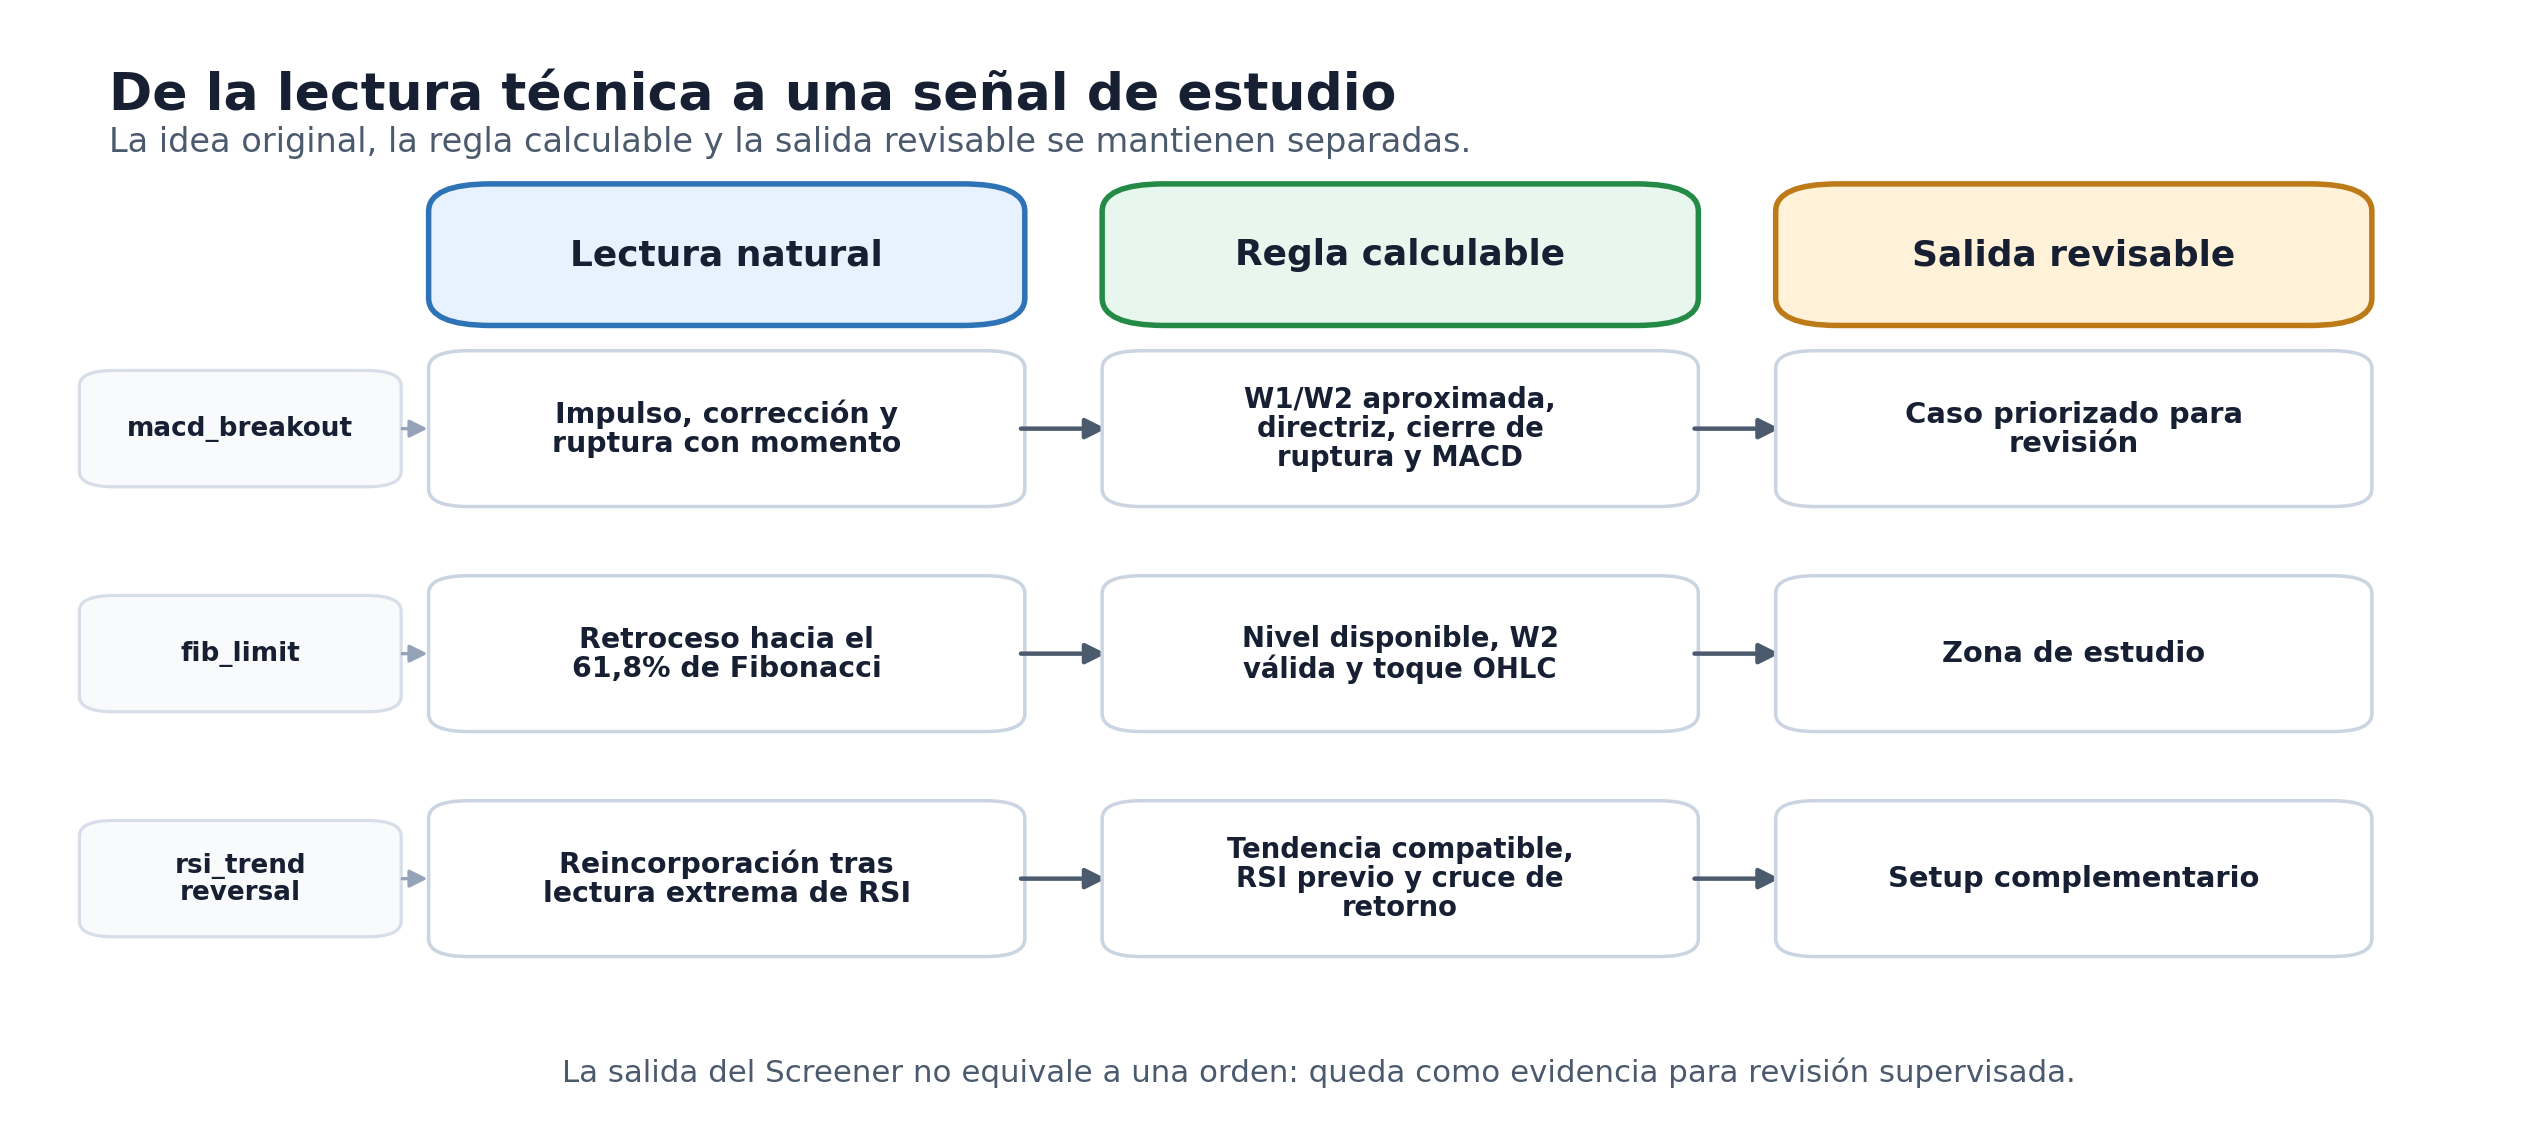
\includegraphics[width=0.98\textwidth]{figs/canonicas/metodologia/formalizacion_setups_flujo_canonico.png}
\caption[Formalizaci\'on de setups y se\~nales de estudio]{Resumen metodol\'ogico del paso entre lectura t\'ecnica, regla
calculable y salida revisable para los setups principales. La figura simplifica
el proceso de formalizaci\'on: una salida del Screener se interpreta como
evidencia de revisi\'on y no como orden autom\'atica ni recomendaci\'on operativa.}
\label{fig:formalizacion-setups-flujo}
\end{figure}

\subsection{Reglas principales formalizadas}
\label{subsec:reglas-principales-formalizadas}

La formalizaci\'on se ha aplicado a tres setups principales. Dos de ellos,
\texttt{macd\_breakout} y \texttt{fib\_limit}, parten de una lectura de ondas:
un impulso inicial, un retroceso posterior y la posibilidad de que el precio
intente continuar el movimiento. El tercero, \texttt{rsi\_trend\_reversal}, es
una regla m\'as simple de reincorporaci\'on a tendencia a partir del RSI. Esta
distinci\'on es importante porque no todas las reglas necesitan la misma
estructura ni producen el mismo tipo de salida.

Para pasar de la lectura visual a una regla calculable se utiliza un paso
intermedio. En las reglas basadas en ondas, la teor\'ia describe impulsos y
correcciones, pero el c\'odigo necesita precios, fechas y niveles concretos.
En esta memoria se usa W1 para referirse al primer tramo impulsivo que sirve de
referencia y W2 para la correcci\'on posterior que no deber\'ia invalidar ese
impulso. Estas etiquetas son una simplificaci\'on operativa para estudiar reglas
con datos, no un conteo completo de Elliott ni una validaci\'on autom\'atica de
la estructura del mercado.

Por eso se utiliza ZigZag como herramienta de aproximaci\'on
\cite{zigzag_jbn_github}. En el proyecto se trabaja con una adaptaci\'on local
de ese enfoque. No forma parte de la teor\'ia de Elliott ni decide por s\'i sola
el conteo. Su funci\'on es ayudar a marcar giros relevantes del precio y a reconstruir
una posible W1 y una posible W2 sobre datos OHLC. A partir de esa estructura,
cada setup define cu\'al es la condici\'on concreta que se quiere estudiar.

\paragraph{\texttt{macd\_breakout}.}
La lectura natural es la de una posible continuaci\'on. Si el precio ha formado
un impulso y despu\'es corrige, la ruptura de la directriz de esa correcci\'on
puede interpretarse como una primera se\~nal de reanudaci\'on. El MACD se a\~nade
como confirmaci\'on de momento: no define la estructura de ondas, pero ayuda a
filtrar rupturas que no van acompa\~nadas por un cambio de impulso suficiente.

\begin{quote}
\small
\textbf{Lectura natural:} posible W1, retroceso W2 y ruptura de la
correcci\'on con apoyo del MACD.\\
\(\Rightarrow\)
\textbf{Regla formalizada:} tendencia compatible, estructura W1/W2 aproximada
por ZigZag, setup activo, ruptura reciente de la directriz W2 y cruce reciente
del MACD en la misma direcci\'on.
\end{quote}

En la implementaci\'on, la ruptura no se dibuja manualmente sobre el gr\'afico.
Se reconstruye a partir de la correcci\'on W2 y se comprueba si el cierre rompe
la directriz estimada. Adem\'as, la ruptura y el cruce del MACD deben aparecer
dentro de una ventana reciente asociada al mismo setup, sin que la estructura
haya quedado invalidada. En backtesting, la entrada se eval\'ua al cierre de la
vela disponible. En el Screener, la misma idea se muestra como setup de estudio
con estado temporal, nivel de ruptura y contexto visual.

En esta regla, el nivel de salida por p\'erdida se sit\'ua en el extremo de la
correcci\'on W2; si ese dato no est\'a disponible, se usa el origen de W1 como
referencia de seguridad. Los objetivos de beneficio se calculan con las
proyecciones 1,0 y 1,618 de la estructura W1/W2. De este modo, entrada, stop y
objetivos quedan ligados a la misma reconstrucci\'on de ondas, y no a una
decisi\'on manual posterior.

\paragraph{\texttt{fib\_limit}.}
La lectura natural no espera la ruptura, sino el retroceso. Tras un impulso
inicial, se estudia si la correcci\'on vuelve a una zona relevante de Fibonacci.
En este trabajo se toma el 61,8\% como nivel principal de revisi\'on, porque
permite convertir una idea visual bastante habitual en una condici\'on concreta:
el precio ha retrocedido hacia una zona t\'ecnica, pero la estructura todav\'ia no
se considera invalidada.

\begin{quote}
\small
\textbf{Lectura natural:} posible W1 y retroceso W2 hacia el 61,8\% de
Fibonacci.\\
\(\Rightarrow\)
\textbf{Regla formalizada:} estructura W1/W2 aproximada por ZigZag, nivel
61,8\% calculado, setup activo, W2 no invalidada y toque del nivel mediante
datos OHLC.
\end{quote}

En las pruebas hist\'oricas, el toque del 61,8\% se utiliza como aproximaci\'on a
una entrada limitada: una compra o venta condicionada a que el precio alcance un
nivel fijado previamente. En posiciones largas (compras), la entrada se
considera activada cuando el m\'inimo de la vela alcanza ese nivel, teniendo en
cuenta el \textit{spread}; en posiciones cortas (ventas), cuando el m\'aximo de la
vela alcanza el nivel equivalente. En ambos casos, la convenci\'on busca que la
activaci\'on sea verificable con la informaci\'on disponible: el nivel de entrada
debe existir antes de la vela evaluada, la estructura debe estar activa antes de
comprobar el toque y el \textit{spread} se tiene en cuenta para no activar una
entrada si el precio de compra o venta correspondiente no habr\'ia alcanzado el
nivel. Adem\'as, el retroceso W2 debe seguir siendo v\'alido dentro de la
estructura Elliott W1/W2 reconstruida; si esa estructura queda invalidada, el
nivel de Fibonacci deja de usarse. En esta regla, el nivel de salida por p\'erdida
se sit\'ua en el origen de W1, mientras que los objetivos de beneficio se toman
de las proyecciones 1,0 y 1,618 calculadas desde el extremo de W2. As\'i, la
entrada, el stop y los objetivos proceden de la misma estructura W1/W2, no de
una decisi\'on manual posterior. En el Screener, la
variante
\texttt{fib\_limit\_live\_candidate} se interpreta de forma m\'as restringida.
Se utiliza para destacar casos en los que el precio se encuentra cerca de una
zona de Fibonacci relevante para la revisi\'on, manteniendo la decisi\'on
operativa fuera del Screener.

\paragraph{\texttt{rsi\_trend\_reversal}.}
Esta regla no intenta reconstruir ondas. Se utiliza como setup complementario
para detectar posibles reincorporaciones a una tendencia ya identificada. La
idea natural es sencilla: en una tendencia alcista, una ca\'ida del RSI a zona de
sobreventa y su posterior recuperaci\'on puede sugerir que el precio vuelve a
acompa\~nar la tendencia. En una tendencia bajista, el caso equivalente aparece
cuando el RSI pasa por sobrecompra y despu\'es vuelve a cruzar hacia abajo.

\begin{quote}
\small
\textbf{Lectura natural:} RSI extremo y vuelta en la direcci\'on de la
tendencia.\\
\(\Rightarrow\)
\textbf{Regla formalizada:} tendencia alineada en varios timeframes,
RSI en zona extrema y cruce de salida del umbral correspondiente: por encima de
30 en tendencia alcista o por debajo de 70 en tendencia bajista.
\end{quote}

Para setups en M15 se exige coherencia con H1 y H4, mientras que para setups en
H1 se revisa la relaci\'on con H4 y D1. Antes del cruce, el sistema puede marcar
un estado de vigilancia cuando el RSI se aproxima a la zona extrema. A
diferencia de \texttt{macd\_breakout} y \texttt{fib\_limit}, esta regla no
define por s\'i sola una estructura completa de stop, objetivo o generaci\'on de
orden; se mantiene como se\~nal de estudio para priorizar revisiones dentro del
Screener.

\begin{table}[H]
\centering
\scriptsize
\setlength{\tabcolsep}{3pt}
\renewcommand{\arraystretch}{1.12}
\begin{tabular}{p{0.20\textwidth}p{0.26\textwidth}p{0.25\textwidth}p{0.21\textwidth}}
\hline
\textbf{Bloque} & \textbf{Par\'ametros principales} & \textbf{Convenci\'on experimental} & \textbf{Lectura en memoria} \\
\hline
\texttt{macd\_breakout} & Estructura W1/W2 aproximada por ZigZag, directriz W2 y confirmaci\'on MACD. & Entrada por ruptura confirmada al cierre; costes incorporados en la simulaci\'on. & Regla principal de ruptura y continuidad. \\
\texttt{fib\_limit} & Nivel 61,8\% de Fibonacci, setup activo, W2 no invalidada y toque OHLC. & Entrada en el nivel cuando, tras crearse el setup, una vela alcanza la zona; stop y objetivo se eval\'uan desde la vela posterior por ambig\"uedad intrabar. & Regla de retroceso; no equivale a orden real enviada. \\
\texttt{rsi\_trend\_reversal} & RSI en zona extrema, salida del umbral y tendencia alineada. & Se usa como se\~nal de estudio del Screener, sin estructura propia de stop y objetivo. & Prioriza revisiones, no forma parte del benchmark principal. \\
Benchmarks de referencia & RSI, bandas de Bollinger, medias m\'oviles y momentum. & Se eval\'uan con el mismo motor, costes y grupos de datos que las reglas principales. & Comparaci\'on frente a reglas simples. \\
M\'etricas y riesgo & Retorno, drawdown, factor de beneficio, expectativa, Sharpe, Sortino, Calmar y Recovery Factor. & Lectura por bloque experimental; no se une todo como una cartera real. & Comparaci\'on de rendimiento y riesgo bajo supuestos comunes. \\
\hline
\end{tabular}
\caption[Par\'ametros y convenciones principales de simulaci\'on]{Resumen compacto de los par\'ametros y convenciones principales usados en la formalizaci\'on y simulaci\'on. La tabla ayuda a reproducir la lectura experimental sin convertir las reglas en instrucciones operativas reales.}
\label{tab:parametros-reglas-simulacion}
\end{table}


La Tabla~\ref{tab:parametros-reglas-simulacion} no sustituye la explicaci\'on
anterior, pero resume las decisiones necesarias para reproducir la lectura
experimental. Su funci\'on es dejar visibles los par\'ametros y convenciones que
condicionan los resultados, especialmente en reglas donde el momento de
activaci\'on, el coste de ejecuci\'on o el control temporal pueden cambiar la
interpretaci\'on del backtest.

\subsection{Contexto y confluencias de revisi\'on}
\label{subsec:contexto-confluencias-revision}

Junto a los setups principales, el sistema calcula capas de contexto destinadas
a facilitar la revisi\'on. Algunas capas describen niveles t\'ecnicos cercanos,
como pivotes, m\'aximos y m\'inimos del d\'ia anterior, n\'umeros redondos o zonas
de Fibonacci contextual. Otras resumen condiciones del mercado o del
indicador, como tendencia, volatilidad o estado del RSI. Tambi\'en se incorpora
la informaci\'on generada por WaveCount y WeaveCount para aportar una lectura
estructural adicional sobre el movimiento del precio.

Estas capas no se interpretan como reglas de entrada independientes. Su papel
es ayudar a responder preguntas de revisi\'on: si el setup aparece cerca de un
nivel relevante, si la direcci\'on coincide con la tendencia de fondo, si existe
una zona de volatilidad elevada o si varios activos podr\'ian estar transmitiendo
informaci\'on similar. Por ejemplo, una zona de Fibonacci contextual puede
aportar una referencia visual para el an\'alisis. No debe confundirse con la
regla \texttt{fib\_limit}; del mismo modo, un nivel de RSI extremo puede
mejorar la lectura de contexto sin convertirse por s\'i solo en una estrategia.

El Screener resume parte de esta informaci\'on mediante etiquetas de confluencia
y una puntuaci\'on de calidad. Esta puntuaci\'on se interpreta como una medida de
claridad para la revisi\'on visual, no como una probabilidad de acierto ni como
una estimaci\'on de rentabilidad esperada. Por ello, una fila con mayor calidad no
significa necesariamente una entrada operativa superior; solo indica que el
caso re\'une m\'as elementos estructurados para ser revisado de forma ordenada.

\subsection{Uso en backtesting y Screener}
\label{subsec:salida-formalizacion-screener}

El resultado de la formalizaci\'on no es una orden de mercado, sino una
representaci\'on intermedia que puede alimentar distintos bloques del TFG. En las pruebas
hist\'oricas, las reglas se convierten en condiciones de entrada, invalidaci\'on,
salida y registro de operaciones. Para el Trading Center, esas mismas ideas se
materializan en filas del Screener con activo, grupo de mercado, timeframe,
direcci\'on, tipo de setup, estado temporal, niveles de referencia, contexto y
campos de auditor\'ia.

Esta representaci\'on mantiene campos expl\'icitos para separar estudio y ejecuci\'on. Los
setups pueden aparecer como casos de revisi\'on, pero no se presentan como
\'ordenes listas para enviar. Cualquier paso posterior hacia generaci\'on de
\'ordenes queda separado en la capa de MT5 Bot y RiskGuard, donde se vuelven a
evaluar condiciones de riesgo, exposici\'on y bloqueo. Esta organizaci\'on
permite que una misma regla sirva para backtesting, visualizaci\'on y an\'alisis
sin mezclar esos usos con una operativa autom\'atica.

La formalizaci\'on cumple as\'i una funci\'on intermedia dentro de la metodolog\'ia.
Convierte una lectura t\'ecnica en datos revisables, pero conserva la prudencia
necesaria para no presentar esos registros como decisiones operativas. En las
secciones posteriores, estas reglas se utilizan para evaluar estrategias,
compararlas con referencias y presentar casos de revisi\'on dentro de la
plataforma interactiva de visualizaci\'on y revisi\'on.

\section{Backtesting, benchmarks y control de sesgos}
\label{sec:backtesting-benchmarks-sesgos}

\subsection{Dise\~no de las pruebas hist\'oricas}
\label{subsec:diseno-pruebas-historicas}

La evaluaci\'on hist\'orica se utiliza para estudiar c\'omo se comportan las
reglas formalizadas cuando se aplican de forma sistem\'atica sobre datos ya
observados. Su funci\'on no es demostrar que una estrategia vaya a ser rentable
en el futuro. Aporta una base cuantitativa para comparar reglas, detectar
debilidades y revisar si una idea t\'ecnica mantiene un comportamiento
razonable bajo una configuraci\'on com\'un. Esta distinci\'on es importante en
sistemas de trading, donde un backtest puede ser \'util como herramienta de
an\'alisis, pero tambi\'en puede inducir conclusiones demasiado optimistas si no
se explican sus supuestos y limitaciones \cite{pardo_2008_trading_strategies,
bailey_etal_2017_backtest_overfitting,lopez_de_prado_2018_afml}.

Este cuidado resulta especialmente importante cuando se optimizan estrategias. En muchos
problemas de ciencia de datos es habitual probar distintas configuraciones y
escoger la que obtiene mejores m\'etricas, siempre que existan controles de
validaci\'on adecuados. En trading, esa pr\'actica requiere una prudencia
adicional: si se prueban miles de combinaciones sobre el mismo hist\'orico,
aumenta la probabilidad de encontrar una regla que encaja por azar en ese
periodo. La mejora observada puede deberse entonces al propio proceso de
b\'usqueda, no a una pauta estable del mercado. Por ese motivo, en este trabajo
la comparaci\'on se plantea con reglas y convenciones previamente fijadas, y las
variantes adicionales se tratan como sensibilidades metodol\'ogicas, no como una
b\'usqueda libre de la configuraci\'on con mejor resultado retrospectivo.
En particular, no se entrena un modelo para ajustar autom\'aticamente los
par\'ametros ni se optimiza una funci\'on objetivo de rentabilidad hist\'orica; las
m\'etricas se usan para evaluar el comportamiento observado bajo una
configuraci\'on definida previamente.

El dise\~no experimental se organiza por bloques independientes. Cada bloque
combina un grupo de activos, como divisas principales, metales o \'indices, con
una configuraci\'on temporal de trabajo: M30:H1, H1:H4 o H4:D1. En M30:H1 y
H1:H4, la primera referencia indica el timeframe operativo y la segunda el contexto
principal; adem\'as, se incorpora el timeframe inmediatamente superior disponible
para reforzar la lectura de tendencia o estructura. En H4:D1, en cambio, la
prueba se documenta como una variante de dos timeframes, porque no se
dispone de un timeframe semanal o mensual dentro del conjunto de datos utilizado.
As\'i, no se fuerza una estructura temporal para la que no existen datos.

En el benchmark principal, el cruce entre tres grupos de activos y tres
configuraciones temporales produce nueve bloques por regla evaluada. Un bloque
no es una operaci\'on individual: es una unidad experimental completa. Dentro de
cada bloque se recorren los activos del grupo, se generan entradas cuando se
cumplen las reglas y se obtiene una curva de resultados para esa configuraci\'on.
Por eso el n\'umero de bloques puede ser reducido y, al mismo tiempo, el n\'umero
de operaciones registradas puede ser elevado.

\begin{table}[H]
\centering
\small
\begin{tabular}{p{0.25\textwidth} p{0.18\textwidth} p{0.42\textwidth}}
\hline
\textbf{Ejemplo de bloque} & \textbf{Configuraci\'on} & \textbf{Lectura experimental} \\
\hline
Divisas principales & M30:H1 & Prueba intradiaria sobre divisas principales; M30 act\'ua como timeframe operativo y H1/H4 aportan contexto. \\
Metales & H1:H4 & Prueba sobre metales con entrada en H1 y contexto superior en H4/D1. \\
\'Indices & H4:D1 & Variante de mayor escala; se usa H4 como timeframe operativo y D1 como contexto disponible. \\
\hline
\end{tabular}
\caption[Ejemplos de bloques experimentales]{Ejemplos de bloques experimentales. Cada bloque combina un grupo de
activos y una configuraci\'on temporal; dentro de \'el pueden aparecer muchas
operaciones, pero las m\'etricas de cartera se interpretan a nivel de bloque.}
\label{tab:ejemplos-bloques-experimentales}
\end{table}

La Tabla~\ref{tab:ejemplos-bloques-experimentales} ayuda a separar visualmente
el bloque experimental de la operaci\'on individual, que es la unidad concreta
registrada dentro de cada bloque.

Las reglas principales evaluadas en esta l\'inea son \texttt{macd\_breakout} y
\texttt{fib\_limit}, junto con una variante combinada usada como referencia
secundaria. No todos los componentes del sistema se incorporan al mismo backtest.
\texttt{rsi\_trend\_reversal} se utiliza como setup de revisi\'on en el Screener,
y WaveCount y WeaveCount se tratan como contexto estructural. Las capas de MT5,
RiskGuard, Telegram y AI Analyst pertenecen a la demostraci\'on, seguimiento y
auditor\'ia del sistema. Esta separaci\'on evita mezclar una evaluaci\'on
hist\'orica de reglas con componentes que tienen una finalidad distinta.

En las estrategias de referencia etiquetadas como 3TF, la condici\'on de entrada
se eval\'ua en el timeframe operativo y se exige que la tendencia sea coherente en
timeframes superiores. Por ejemplo, en M30:H1 la entrada se revisa sobre M30 y el
contexto se obtiene de H1 y H4; en H1:H4 se usa H1 como timeframe operativo y H4/D1
como contexto; en H4:D1 la comparaci\'on queda limitada a H4 y D1, porque D1 es
el timeframe superior disponible en el conjunto de datos. Esta lectura 3TF act\'ua
como filtro de alineaci\'on temporal, no como una estrategia adicional distinta.

\subsection{Control temporal y convenciones de simulaci\'on}
\label{subsec:control-temporal-backtesting}

En una prueba hist\'orica de trading no basta con comprobar si una regla se
cumple en el gr\'afico. Tambi\'en hay que asegurar que la decisi\'on simulada solo
usa informaci\'on que habr\'ia estado disponible en ese momento. En este trabajo,
ese control empieza en la preparaci\'on de los datos: la ingesta trabaja con
velas cerradas y el backtest eval\'ua las condiciones de entrada sobre datos
OHLC ya formados. Con ello se reduce el riesgo de \textit{look-ahead}, es
decir, el uso de informaci\'on futura dentro de una evaluaci\'on retrospectiva.

Este control es especialmente importante en las reglas que dependen de
estructura. La reconstrucci\'on W1/W2 no se da por v\'alida solo porque el precio
haya dibujado un extremo visual, sino cuando ese extremo queda confirmado por
el proceso de ZigZag. Adem\'as, la desviaci\'on din\'amica del ZigZag se calcula
sin utilizar la vela que se est\'a evaluando en ese instante. La tendencia del
timeframe superior tambi\'en se sincroniza para que el timeframe operativo solo
pueda usar velas superiores ya cerradas. En \texttt{fib\_limit}, el toque del 61,8\% se
eval\'ua \'unicamente si el setup ya estaba activo antes de esa vela; de este
modo, una estructura reci\'en identificada no se convierte inmediatamente en una
entrada simulada.

Para evitar que el propio par\'ametro del ZigZag incorpore informaci\'on futura,
la desviaci\'on se estima mediante una mediana expansiva de volatilidad relativa,
basada en ATR/precio. Esta desviaci\'on se calcula con la informaci\'on disponible
hasta la vela anterior antes de evaluar la estructura actual.
Adem\'as, los pivotes detectados por ZigZag no se tratan como disponibles en el
instante del extremo, sino cuando el movimiento posterior confirma el giro. De
este modo, el umbral usado para reconstruir W1/W2 se adapta al activo y al grupo
de mercado, pero la estructura solo se utiliza cuando habr\'ia estado disponible
en una simulaci\'on que respeta el orden temporal.

A partir de esa base temporal, cada tipo de entrada se modela con una
convenci\'on concreta. En las reglas de ruptura, la entrada se eval\'ua al cierre
de la vela del timeframe operativo. En \texttt{macd\_breakout}, la directriz de la
correcci\'on W2 se construye con m\'aximos en posiciones largas y m\'inimos en
posiciones cortas, y la confirmaci\'on exige que el cierre de la vela cruce esa
directriz. Esta convenci\'on evita que una mecha aislada se trate como una
ruptura confirmada.

En \texttt{fib\_limit}, la entrada se modela de forma distinta. La regla
representa una orden limitada situada previamente en el nivel 61,8\% de
Fibonacci, es decir, una orden que solo se activar\'ia si el precio llega al nivel
definido. Si una vela posterior a la creaci\'on del setup alcanza ese nivel por
el lado correspondiente, el backtest registra la entrada en esa misma vela y al
precio del nivel. Por tanto, la entrada no se desplaza a la apertura de la vela
siguiente. La limitaci\'on aparece despu\'es: con datos OHLC se sabe que el nivel
ha sido alcanzado dentro de la vela, pero no el orden exacto de los movimientos
internos.

La ambig\"uedad intrabar se trata mediante convenciones fijas. Para posiciones
ya activas, si stop y objetivo podr\'ian alcanzarse dentro de la misma vela, el
criterio prioriza el stop. En la vela de entrada de \texttt{fib\_limit}, en
cambio, no se eval\'uan stop ni objetivo. El motivo es que el OHLC solo resume
apertura, m\'aximo, m\'inimo y cierre, pero no indica si, despu\'es de activar la
entrada, el precio toc\'o primero el stop, el objetivo o ninguno de los dos. Para
no introducir una secuencia interna no observada en los datos, la gesti\'on de
salida empieza desde la vela posterior a la entrada. Esta segunda convenci\'on no
se interpreta como una regla necesariamente favorable o desfavorable, sino como
una decisi\'on metodol\'ogica derivada de la granularidad disponible.

Estas convenciones no pretenden reproducir todos los detalles de una ejecuci\'on
real. El backtest incorpora costes como \textit{spread} y comisiones, pero no
modela otros elementos como el \textit{swap}, el deslizamiento adicional en
movimientos r\'apidos, la prioridad de ejecuci\'on o las ejecuciones parciales.
Por ello, los resultados deben leerse como una evaluaci\'on metodol\'ogica de las
reglas, no como una reproducci\'on completa de todas las condiciones de una
operaci\'on real.

\subsection{Benchmarks de comparaci\'on}
\label{subsec:benchmarks-comparacion}

Una estrategia no se eval\'ua de forma aislada, sino frente a referencias
simples y comparables. Para ello se utilizan benchmarks cl\'asicos basados en
ideas conocidas de an\'alisis t\'ecnico: reversi\'on a la media con RSI, reentrada
de momento con RSI, cruce de medias y reentrada mediante bandas de Bollinger
\cite{wilder_1978_new_concepts,murphy_1999_technical_analysis,
bollinger_2001_bands}. Estas reglas no se plantean como alternativas
optimizadas ni como estrategias finales, sino como puntos de comparaci\'on
explicables.

La comparaci\'on reutiliza la misma estructura experimental que las reglas
principales:
datos procesados, grupos de activos, timeframes, costes, tama\~no de
posici\'on, esquema de registro de operaciones y divisiones temporales. De esta
forma, la comparaci\'on no queda condicionada por diferencias en el motor de
simulaci\'on utilizado para cada regla. El objetivo es que \texttt{macd\_breakout} y
\texttt{fib\_limit} puedan leerse en relaci\'on con reglas de referencia bajo un
marco com\'un, no solo a partir de sus resultados absolutos.

\subsection{Salidas, m\'etricas y lectura de resultados}
\label{subsec:salidas-metricas-backtesting}

Cada ejecuci\'on del experimento genera salidas revisables: metadatos de configuraci\'on,
registros de operaciones, tablas de m\'etricas, auditor\'ias de riesgo y figuras
de resumen. Estas salidas permiten comprobar qu\'e datos se usaron, qu\'e regla
produjo cada entrada, cu\'al fue la salida registrada y bajo qu\'e supuestos se
calcul\'o el resultado. En lugar de depender de una lectura manual posterior, el
flujo conserva evidencias que pueden revisarse desde distintas perspectivas:
por estrategia, por grupo de activos, por timeframe y por bloque
experimental.

Para interpretar estas salidas se distinguen tres niveles. El primero es el
bloque experimental, formado por una combinaci\'on concreta de grupo de activos
y timeframe. En ese nivel se calculan m\'etricas como retorno, drawdown,
Sharpe, Sortino o Calmar, porque cada bloque se analiza como una prueba
separada. El segundo nivel resume los resultados entre bloques y sirve para
comparar tendencias generales, pero no equivale a unir todas las operaciones en
una sola simulaci\'on conjunta. El tercer nivel corresponde al registro de
operaciones, que permite revisar n\'umero de operaciones, factor de beneficio,
expectativa o resultado por operaci\'on. Por tanto, cada tabla se utiliza para
una lectura distinta: evoluci\'on dentro de cada prueba, comparaci\'on general
entre pruebas y detalle de las entradas y salidas registradas.

Las m\'etricas principales se calculan a partir del registro de operaciones y
de una serie temporal de capital simulada para cada bloque. En este trabajo,
esa serie no se actualiza vela a vela, sino cada vez que una o varias
operaciones finalizan. En cada evento de salida se suma el resultado observado
y se obtiene un nuevo punto de la serie. Por tanto, el drawdown se calcula
sobre esa secuencia discreta de valores ya observados, y no sobre la posible
variaci\'on provisional de una operaci\'on mientras permanece abierta. Para fijar la notaci\'on, \(E_0\) es el capital
inicial, \(E_T\) el capital final y \(E_t\) la curva de capital tras cada
evento de salida. El retorno de cada evento se denota como \(r_t\).
\(g_i\) representa el resultado monetario de la operaci\'on \(i\), y \(N\) es el
n\'umero total de operaciones. Adem\'as, \(N_+\) indica las operaciones con resultado positivo, y
\(n\) el n\'umero de eventos de salida del bloque usado como factor de escala
interno en las razones entre retorno y riesgo.
En estas razones, \(\overline{r}\) representa el retorno medio por evento y
\(\sigma(\cdot)\) la desviaci\'on t\'ipica correspondiente.
Para Sortino, \(\sigma_-(r)\) representa la desviaci\'on t\'ipica calculada
solo sobre los retornos negativos.
Cuando se normaliza el resultado por operaci\'on, \(\rho_i\) representa el
riesgo monetario inicial asumido en la operaci\'on \(i\).
Para la exposici\'on temporal, \(\Delta t_i\) representa la duraci\'on de la
operaci\'on \(i\), y \(T_\text{bloque}\) la ventana temporal total cubierta por
el bloque experimental.
Para la m\'etrica Calmar, \(R_\text{anualizado}\) representa el retorno
anualizado del bloque y \(DD_\text{max}\) el drawdown m\'aximo observado. Con
esta notaci\'on, las definiciones usadas en la lectura de resultados son las
recogidas en la
Tabla~\ref{tab:definicion-metricas-backtesting}.

\begin{table}[H]
\centering
\scriptsize
\setlength{\tabcolsep}{4pt}
\renewcommand{\arraystretch}{1.13}
\begin{tabular}{p{0.19\textwidth} p{0.31\textwidth} p{0.40\textwidth}}
\hline
\textbf{M\'etrica} & \textbf{Definici\'on matem\'atica} & \textbf{Interpretaci\'on conceptual y financiera} \\
\hline
Retorno & \(R = \left(\frac{E_T}{E_0}-1\right)\cdot 100\) & Variaci\'on del capital simulado del bloque; indica si la prueba termina con ganancia o p\'erdida. \\
Drawdown m\'aximo & \(\max_t \left(\frac{\max_{\tau \leq t} E_\tau - E_t}{\max_{\tau \leq t} E_\tau}\right)\cdot 100\) & Mayor descenso relativo entre un m\'aximo previo y un punto posterior de la serie de capital simulada. \\
Aciertos & \(\frac{N_+}{N}\cdot 100\) & Proporci\'on de operaciones positivas; no basta por s\'i sola si las p\'erdidas son mayores que las ganancias. \\
Factor de beneficio & \(\frac{\sum_{g_i>0} g_i}{|\sum_{g_i\leq 0} g_i|}\) & Relaci\'on entre ganancias y p\'erdidas brutas; valores superiores a 1 indican que las ganancias agregadas superan a las p\'erdidas. \\
Expectativa & \(\frac{1}{N}\sum_{i=1}^{N} g_i\) & Resultado medio por operaci\'on; resume si una operaci\'on promedio aporta o destruye valor bajo esas reglas. \\
Expectativa en riesgo & \(\frac{1}{N}\sum_{i=1}^{N}\frac{g_i}{\rho_i}\) & Resultado medio por operaci\'on medido en unidades de riesgo inicial; facilita comparar reglas con tama\~nos de stop distintos. \\
Exposici\'on temporal & \(\frac{\sum_i \Delta t_i}{T_\text{bloque}}\cdot 100\) & Proporci\'on agregada de tiempo con operaciones abiertas; puede superar el 100\% cuando varias posiciones coinciden en el tiempo. \\
Sharpe & \(\frac{\overline{r}}{\sigma(r)}\sqrt{n}\) & Retorno medio dividido por la volatilidad total; pregunta si el retorno compensa la variabilidad asumida. \\
Sortino & \(\frac{\overline{r}}{\sigma_-(r)}\sqrt{n}\) & Retorno medio dividido por la volatilidad negativa; penaliza con mayor foco las desviaciones desfavorables. \\
Calmar & \(\frac{R_\text{anualizado}}{DD_\text{max}}\) & Relaci\'on entre crecimiento anualizado y peor ca\'ida; eval\'ua si el retorno compensa el drawdown asumido. \\
Recovery Factor & \(\frac{R}{DD_\text{max}}\), con \(DD_\text{max}>0\) & Retorno final por unidad de drawdown m\'aximo; en esta memoria se interpreta a nivel de bloque, no como una cartera global. \\
\hline
\end{tabular}
\caption[Definici\'on de m\'etricas de backtesting]{Definici\'on de las m\'etricas principales utilizadas en los backtests.
Las m\'etricas de curva se interpretan a nivel de bloque experimental; las
m\'etricas por operaci\'on complementan esa lectura, pero no sustituyen el
an\'alisis de riesgo agregado del bloque.}
\label{tab:definicion-metricas-backtesting}
\end{table}

Las definiciones anteriores tambi\'en requieren convenciones para casos l\'imite.
Si un bloque no contiene operaciones, las m\'etricas por operaci\'on no tienen
lectura econ\'omica. Si no hay p\'erdidas, el factor de beneficio queda
formalmente no acotado y no debe interpretarse como robustez por s\'i solo. Del
mismo modo, Sharpe y Sortino dejan de ser informativos cuando la desviaci\'on
t\'ipica correspondiente es nula, y Calmar o Recovery Factor no son comparables
cuando el drawdown m\'aximo es cero. En esta memoria, Sharpe y Sortino se usan
como \'indices internos basados en eventos de salida del bloque, no como ratios
anualizados de una serie temporal homog\'enea de retornos diarios.

Estas m\'etricas no tienen el mismo significado. El retorno y el drawdown
describen la evoluci\'on de una prueba completa. Sharpe, Sortino, Calmar y
Recovery Factor ayudan a comparar retorno y riesgo dentro de esa misma curva.
La tasa de acierto, el factor de beneficio y las dos formas de expectativa
resumen el comportamiento de las operaciones individuales.
Por este motivo, una estrategia puede tener muchas operaciones ganadoras y aun
as\'i presentar una curva poco atractiva si sus p\'erdidas son grandes, si el
drawdown es elevado o si el resultado se concentra en pocos bloques.
Las razones ajustadas al riesgo se utilizan, por tanto, como indicadores
comparativos dentro del dise\~no experimental del TFG. No deben interpretarse
como una estimaci\'on universal de rendimiento anualizado ni como una medida de
robustez fuera de los datos y reglas utilizados.

Esta lectura condiciona el modo en que se presentan los resultados en el
cap\'itulo siguiente. Las cifras se utilizan para describir el comportamiento
observado en los experimentos realizados, no para afirmar rentabilidad futura
ni robustez fuera del conjunto evaluado. Por ello, las tablas y figuras se
acompa\~nan de cautelas sobre bloques independientes, dispersi\'on entre grupos,
convenciones de ejecuci\'on y riesgo de sobreajuste. El valor principal del
backtesting en este TFG es que transforma reglas discrecionales en pruebas
revisables y comparables, manteniendo visibles los l\'imites de esa evaluaci\'on.

\section{Formalizaci\'on experimental del enfoque Men\'endez}
\label{sec:formalizacion-menendez}

\subsection{Papel de Men\'endez dentro del TFG}
\label{subsec:papel-menendez-tfg}

El enfoque de Men\'endez Larre se incorpora como una l\'inea de trabajo
experimental dentro del TFG. Su inter\'es dentro de la memoria no se limita a
generar entradas para una estrategia. Tambi\'en permite estudiar una lectura
m\'as detallada de Elliott, apoyada en fractalidad, Parabolic SAR (PSAR),
filtros de tendencia, indicadores de momento y relaciones entre marcos
temporales. El PSAR se entiende aqu\'i como un indicador que marca cambios de
tramo mediante puntos de seguimiento. Esa
misma riqueza hace que la formalizaci\'on sea m\'as delicada, porque una parte de
la interpretaci\'on original depende del criterio visual y de decisiones de
contexto.

Por ese motivo, Men\'endez no se utiliza como eje principal de la comparaci\'on
emp\'irica. El objetivo de esta l\'inea no es demostrar que la metodolog\'ia sea
rentable en general, ni ajustar sus reglas hasta obtener un resultado favorable.
Lo que se busca es comprobar hasta qu\'e punto una lectura t\'ecnica m\'as
discrecional puede transformarse en un flujo de reglas, registros y pruebas
revisables.

Esta decisi\'on permite mantener separadas dos preguntas distintas. La primera
es si las estrategias principales formalizadas en la secci\'on anterior se
comportan de forma competitiva frente a reglas de referencia. La segunda es qu\'e
ocurre cuando se intenta mecanizar una lectura Elliott m\'as compleja. Men\'endez
se sit\'ua en esta segunda pregunta: aporta un caso de estudio sobre
formalizaci\'on, pero no se presenta como estrategia final robusta.

\subsection{Traducci\'on de la lectura visual a capas calculables}
\label{subsec:menendez-variantes-operables}

La formalizaci\'on parte de una relaci\'on entre un timeframe superior y un
timeframe operativo. En esta implementaci\'on, H4 se emplea como contexto y M30 como
timeframe de entrada. A partir de esa relaci\'on se separan tres elementos: el filtro
de tendencia, la lectura de la correcci\'on y la condici\'on que permitir\'ia
activar una entrada simulada.

La idea natural que se intenta trasladar a reglas calculables es la siguiente:
si el timeframe superior mantiene una direcci\'on compatible, se busca en el timeframe
operativo una correcci\'on que pueda interpretarse como una pausa dentro de un
movimiento mayor. La entrada no se plantea por la aparici\'on aislada de un
indicador, sino por la combinaci\'on de contexto, estructura, zona t\'ecnica y
activaci\'on. Esta diferencia es importante porque la lectura original se apoya
en varias capas que, al programarse, deben separarse para poder auditar cada
decisi\'on.

La estructura buscada no consiste en validar retrospectivamente tres ondas
completas, sino en reconocer un movimiento impulsivo previo, estudiar su
correcci\'on y evaluar si aparecen condiciones que permitan plantear una posible
continuaci\'on. Este matiz es importante porque, si se esperase a confirmar por
completo el nuevo tramo impulsivo, la entrada pasar\'ia a depender de informaci\'on
posterior.

La primera capa corresponde al sesgo del timeframe superior. En la formalizaci\'on,
la media m\'ovil simple de 200 periodos (SMA200) se utiliza como filtro principal
de tendencia en H4. El abanico de medias de menor periodo, especialmente 5, 8,
13 y 21, sirve para describir la fuerza y el orden interno del movimiento. Esta parte no genera por s\'i sola una entrada, pero ayuda a
decidir si tiene sentido buscar continuaci\'on o si el contexto es demasiado
ambiguo. La segunda capa aproxima la correcci\'on: el PSAR se utiliza como
herramienta de segmentaci\'on mec\'anica para dividir el precio en
tramos y localizar giros relevantes. Esta segmentaci\'on no pretende confirmar de
forma definitiva un conteo Elliott, sino crear una versi\'on revisable de una
lectura que originalmente es visual.

Sobre esa correcci\'on se incorporan niveles de Fibonacci, zonas de invalidaci\'on
y objetivos. En la l\'ogica de la estrategia, Fibonacci ayuda a situar el
retroceso y las extensiones posibles, mientras que el extremo de la correcci\'on
act\'ua como referencia natural para el riesgo. La activaci\'on se estudia despu\'es
mediante un disparador de entrada, como la ruptura del abanico de medias o el
cambio de tramo indicado por el PSAR. Los indicadores de momento, como MACD o
estoc\'astico, se utilizan como confirmaci\'on adicional y no como sustitutos de
la estructura.
La Figura~\ref{fig:menendez-capas-formalizacion} resume esta separaci\'on en
capas calculables.

\begin{figure}[!htbp]
\centering
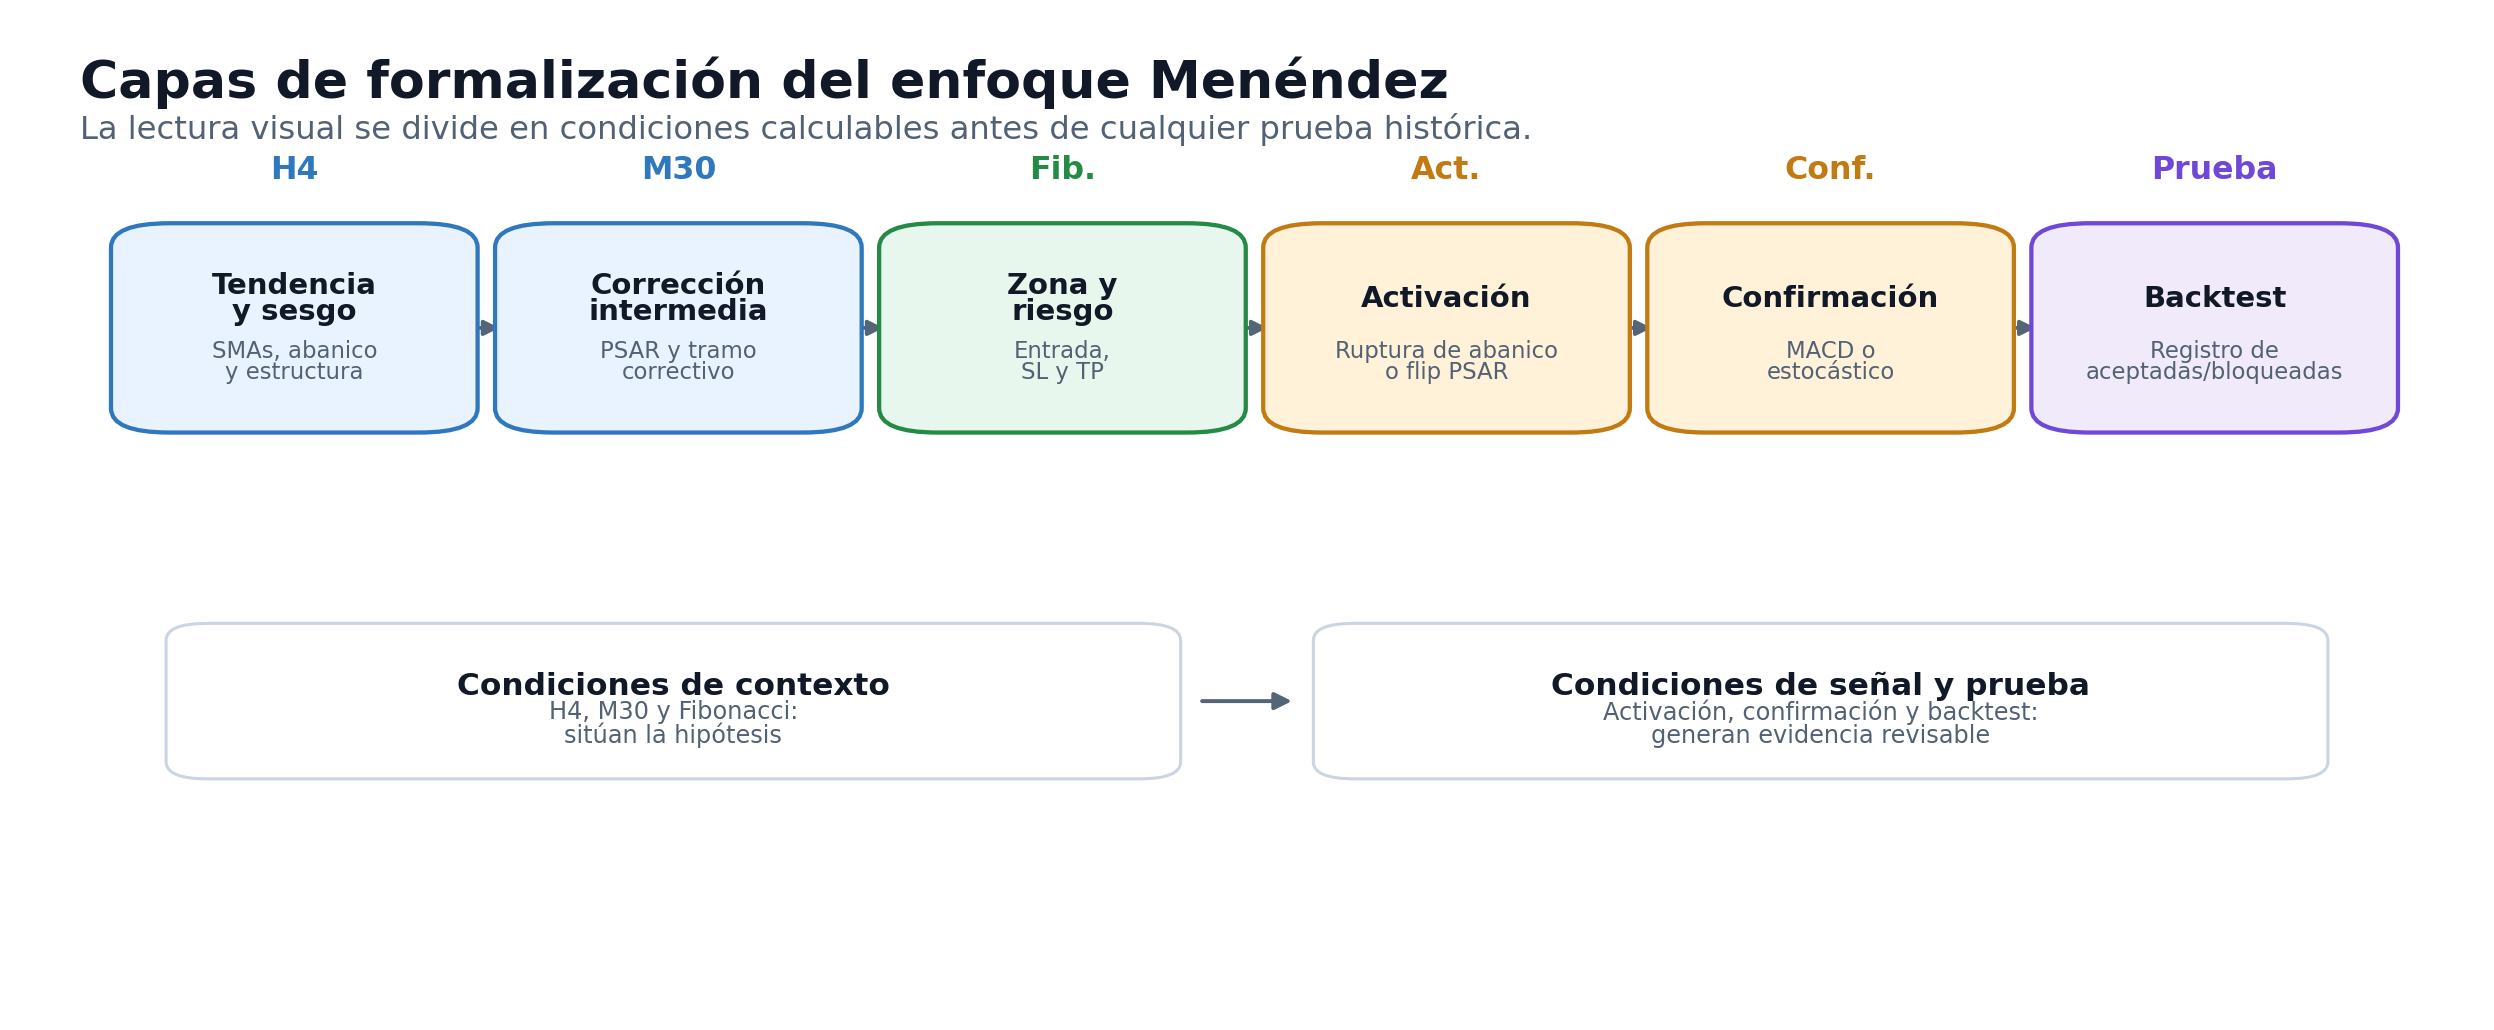
\includegraphics[width=0.98\textwidth]{figs/canonicas/metodologia/menendez_capas_canonico.png}
\caption[Capas de formalizaci\'on del enfoque Men\'endez]{Capas utilizadas para traducir el enfoque Men\'endez a condiciones
calculables. El esquema separa contexto, correcci\'on, zona de riesgo,
activaci\'on, confirmaci\'on y prueba hist\'orica; no representa una secuencia
autom\'atica de ejecuci\'on real.}
\label{fig:menendez-capas-formalizacion}
\end{figure}

A partir de estas capas se definieron varias variantes. La variante principal
mantiene una jerarqu\'ia m\'as cercana al planteamiento de partida: SMA200 como
filtro principal de tendencia, segmentaci\'on mediante PSAR, activaci\'on por ruptura
o cambio de tramo y confirmaci\'on de momento. Una segunda variante relaja parte
de la simultaneidad entre disparadores para estudiar si una lectura demasiado
r\'igida estaba descartando casi todos los casos. Por \'ultimo, la variante
exploratoria de correcci\'on compuesta permite representar correcciones en las que
el retroceso no queda reducido a un \'unico movimiento correctivo, sino a una
secuencia ABC construida con varios segmentos PSAR. En este caso, la secuencia
ABC describe la correcci\'on intermedia, no todo el patr\'on de impulso,
correcci\'on y continuaci\'on. Esta variante se aproxima mejor a correcciones
m\'as complejas dentro de una lectura Elliott, pero tambi\'en a\~nade m\'as
decisiones intermedias y resulta m\'as dif\'icil de validar mec\'anicamente.
Los nombres internos de estas variantes se mantienen en las tablas por
trazabilidad, pero en la memoria se interpretan por su funci\'on metodol\'ogica.

Esta organizaci\'on evita mezclar todas las decisiones en una regla opaca. Si
una variante apenas genera entradas, esa salida no se corrige forzando nuevas
condiciones, sino que se conserva como parte de la evidencia. En una lectura de
este tipo, que el proceso reduzca mucho el n\'umero de casos tambi\'en informa
sobre la dificultad de convertir una teor\'ia visual en condiciones mec\'anicas
reproducibles.

\subsection{Embudo de validaci\'on y lectura de resultados}
\label{subsec:menendez-embudo-validacion}

La evaluaci\'on de esta l\'inea se organiza como un embudo porque cada capa puede
descartar un caso antes de llegar a una entrada simulada. Primero se comprueba
si el contexto H4 es compatible con la direcci\'on buscada. Despu\'es se revisa si
la segmentaci\'on por PSAR permite identificar una correcci\'on interpretable y si
esa correcci\'on encaja con los niveles t\'ecnicos utilizados para estudiar
retroceso, invalidaci\'on y objetivo. Solo a partir de ah\'i se eval\'uan los
disparadores de entrada y las confirmaciones de momento.

El cierre emp\'irico se realiz\'o sobre un conjunto acotado de divisas
principales, con H4 como timeframe superior y M30 como timeframe operativo, y con
variantes definidas antes de revisar los resultados. Esta decisi\'on evita
convertir el proceso en una b\'usqueda libre de par\'ametros. La funci\'on de la
prueba no es adaptar la teor\'ia al hist\'orico disponible, sino observar c\'omo se
comporta una formalizaci\'on previamente fijada.

El embudo tambi\'en ayuda a interpretar los resultados sin reducir toda la
l\'inea a una \'unica cifra final. Si una variante genera pocos casos, el registro
permite distinguir si el problema aparece en el contexto, en la identificaci\'on
de la correcci\'on, en la activaci\'on de la entrada, en la confirmaci\'on de
momento o en la relaci\'on entre riesgo y objetivo. Esta lectura resulta
especialmente \'util en una metodolog\'ia que parte de criterios visuales y los
convierte en reglas calculables, porque permite saber qu\'e parte de la
formalizaci\'on limita el paso de una hip\'otesis visual a una prueba hist\'orica.

\subsection{Alcance final de la l\'inea Men\'endez}
\label{subsec:alcance-final-menendez}

La l\'inea Men\'endez queda, por tanto, como un bloque metodol\'ogico cerrado. No
se presenta como evidencia de rentabilidad ni como una segunda l\'inea emp\'irica
favorable. Su aportaci\'on principal es mostrar el proceso de traducci\'on de una
lectura t\'ecnica compleja a reglas revisables, con variantes separadas y un
registro expl\'icito de las etapas intermedias.

Esta lectura tambi\'en conecta con el resto del TFG. La separaci\'on entre
contexto, setup, prueba hist\'orica y posible uso operativo no se introduce solo
por esta l\'inea, sino como criterio general del proyecto. En el caso de
Men\'endez resulta especialmente visible porque la formalizaci\'on obliga a
distinguir entre una lectura de mercado, una condici\'on calculable, una prueba
hist\'orica y una decisi\'on que, en este trabajo, no se automatiza en real.

En los resultados, Men\'endez se leer\'a como un caso de estudio metodol\'ogico,
no como una demostraci\'on de sistema listo para operar. Este alcance permite
aprovechar la informaci\'on que aporta la prueba sin sobreinterpretarla y deja
las posibles mejoras de la formalizaci\'on como una l\'inea razonable de trabajo
futuro.

\section[An\'alisis estructural con WaveCount y WeaveCount]{An\'alisis estructural con WaveCount y\\ WeaveCount}
\label{sec:wavecount-weavecount-metodologia}

\subsection{Prop\'osito de la capa estructural}
\label{subsec:proposito-capa-estructural}

El backtesting permite evaluar reglas concretas de entrada y salida, pero no
describe por s\'i solo c\'omo est\'a organizado el movimiento reciente del precio.
En un trabajo basado en Elliott y fractalidad, esa lectura estructural tambi\'en
resulta relevante: puede indicar si el precio muestra impulsos claros,
correcciones, tramos ambiguos o zonas donde la interpretaci\'on visual es poco
estable. Esta informaci\'on no se plantea como una estrategia adicional, sino
como una capa de contexto para ordenar la revisi\'on.

En la memoria se distinguen dos conceptos relacionados. WaveCount representa la
l\'inea metodol\'ogica dedicada a convertir una lectura visual de ondas en estados
calculables sobre velas. WeaveCount es la aplicaci\'on de esa idea dentro del
Trading Center, donde se muestran hip\'otesis estructurales sobre activos y
timeframes concretos. La distinci\'on es importante porque evita tratar
el conteo como una lectura definitiva del mercado.

La funci\'on de esta capa es complementar el Screener, no sustituirlo. Un setup
puede indicar que se ha cumplido una regla formalizada, mientras que la lectura
estructural ayuda a revisar si el movimiento reciente tiene una organizaci\'on
compatible con una hip\'otesis de impulso, correcci\'on o continuidad. Esa
informaci\'on puede mejorar la revisi\'on visual del caso, pero no cambia por s\'i
sola la salida de la regla ni habilita ning\'un paso operativo.

\subsection{Criterio de conteo y estados candidatos}
\label{subsec:criterio-conteo-estados}

La lectura de ondas presenta una dificultad propia: el conteo puede cambiar
seg\'un la escala temporal, el punto de origen elegido o la importancia asignada
a cada giro del precio. Por ese motivo, la metodolog\'ia no fuerza un conteo
completo en todos los casos. La capa estructural trabaja con swings y pivotes
confirmables, y permite clasificar un tramo como candidato, ambiguo, invalidado
o insuficientemente claro.

Esta decisi\'on tambi\'en responde al control temporal del trabajo. Un extremo del
precio puede parecer evidente al mirar el gr\'afico completo, pero eso no
significa que estuviera confirmado cuando ocurri\'o. Por ello se diferencia el
momento en que aparece el extremo del momento en que puede considerarse
detectado. Esta separaci\'on evita utilizar una estructura conocida
retrospectivamente como si hubiera estado disponible desde el principio.

En WeaveCount, las etiquetas visibles se leen como hip\'otesis de estudio. Una
marca como W2? o W3? indica que el sistema ha encontrado una estructura
compatible con esa fase, pero todav\'ia no representa una confirmaci\'on
operativa. El signo de interrogaci\'on se mantiene de forma deliberada: expresa
incertidumbre y recuerda que el conteo se ofrece para revisi\'on visual.
Estas etiquetas pertenecen a la capa estructural y no deben identificarse de
forma autom\'atica con la W1/W2 operativa usada en las reglas del benchmark. En
el benchmark, W1/W2 es una simplificaci\'on para construir niveles y directrices
de entrada; en WeaveCount, W2?, W3?, W4? o W5? son hip\'otesis visuales de una
escala concreta y se mantienen como material de revisi\'on.

Adem\'as de la geometr\'ia del conteo, durante el desarrollo se revisaron apoyos
cuantitativos de momentum, como el Elliott Wave Oscillator (EWO) 5-35, para
valorar si ayudaban a interpretar el papel de algunas ondas. Este indicador
puede aportar contexto
sobre la fuerza relativa de una onda tercera o la p\'erdida de momentum en una
posible quinta onda. Tambi\'en permite observar diferencias entre la evoluci\'on
del precio y del oscilador compatibles con una posible divergencia. Sin embargo,
no se utiliza como filtro duro ni como se\~nal autom\'atica, ya que su escala no
est\'a acotada y var\'ia entre activos. Normalizarlo con la muestra disponible
habr\'ia introducido una dependencia fr\'agil: un dato futuro fuera de la escala
observada podr\'ia alterar la interpretaci\'on del indicador. Por ello, en este
TFG se conserva como apoyo de contexto para acompa\~nar la revisi\'on estructural,
no como regla de decisi\'on.

Convertir estas lecturas de momentum o divergencia en reglas robustas requerir\'ia
una validaci\'on espec\'ifica por activo, timeframe y r\'egimen de mercado.

\subsection{Calidad visual y revisi\'on en la plataforma}
\label{subsec:calidad-visual-plataforma}

Para que esta capa sea \'util en una pantalla de revisi\'on, no basta con mostrar
una etiqueta de onda. Tambi\'en conviene indicar si la hip\'otesis tiene soporte
visual suficiente. Por eso WeaveCount incorpora una clasificaci\'on de calidad
orientada a priorizar la revisi\'on: fuerte, media o d\'ebil. Esta calidad no
representa probabilidad de acierto, rentabilidad esperada ni ventaja
estad\'istica; solo resume si la estructura detectada se ve m\'as o menos clara
en el corte analizado.

La calidad se apoya en criterios visuales y estructurales, como la madurez del
tramo, el peso del movimiento actual frente al rango observado, la
disponibilidad de niveles relevantes y la claridad de los puntos de estructura.
Si el soporte es limitado, el caso puede seguir apareciendo como candidato, pero
debe interpretarse con cautela. Esta organizaci\'on permite distinguir entre
casos que merecen una revisi\'on m\'as directa y casos que solo aportan contexto
d\'ebil o incompleto.

En la plataforma, WeaveCount se presenta como una vista visual de estudio.
Permite filtrar por timeframe, grupo de activos, direcci\'on y calidad, y
abrir gr\'aficos con velas, tramos previos, tramo actual y niveles estructurales
cuando est\'an disponibles. La finalidad de esta vista es hacer visible la
hip\'otesis de conteo y sus cautelas para revisarla junto al resto de informaci\'on
del Trading Center.

\subsection{L\'imites de uso y relaci\'on con el resto del sistema}
\label{subsec:limites-wavecount-weavecount}

La capa estructural se mantiene separada de las decisiones operativas. Sus
salidas no alimentan RiskGuard como filtro obligatorio, no activan Telegram, no
conectan con MT5 y no modifican las reglas evaluadas en backtesting. Esta
separaci\'on es necesaria porque una estructura visualmente legible no implica
por s\'i sola una ventaja rentable ni una condici\'on de riesgo aceptable.

Tampoco se utiliza esta capa como demostraci\'on de robustez financiera. Que un
tramo pueda etiquetarse como W2?, W3? o W4? solo significa que se ha encontrado
una hip\'otesis estructural bajo los criterios definidos. Para afirmar que esa
informaci\'on mejora una estrategia har\'ia falta una evaluaci\'on posterior
espec\'ifica, con dise\~no experimental propio y controles de sesgo. En esta
memoria, por tanto, se presenta como contexto estructural y herramienta de
revisi\'on.

Su valor dentro del TFG est\'a en hacer expl\'icita una lectura que, de otro modo,
quedar\'ia como interpretaci\'on visual aislada. Al combinarse con setups, niveles
t\'ecnicos, tendencia, volatilidad y visualizaciones del dashboard, ayuda a
ordenar la revisi\'on del mercado y a hacer m\'as directa la primera lectura de
los motivos por los que un caso puede resultar interesante, sin convertir esa
lectura en una se\~nal autom\'atica.

\section{Arquitectura basada en archivos de evidencia y actualizaci\'on}
\label{sec:arquitectura-artifact-first-refresh}

\subsection{Papel de los archivos de evidencia en la metodolog\'ia}
\label{subsec:papel-artifacts-metodologia}

La metodolog\'ia del TFG no consiste solo en ejecutar scripts o visualizar el
resultado final en el dashboard. Cada bloque relevante produce salidas
intermedias que pueden revisarse de forma independiente: tablas CSV, ficheros
JSON, informes, capturas, auditor\'ias y manifiestos. En esta memoria se usa el
t\'ermino \textit{artifact} para referirse a esas salidas guardadas que permiten
saber qu\'e se gener\'o, con qu\'e datos y bajo qu\'e condiciones.

Esta decisi\'on tiene una funci\'on metodol\'ogica. Si el resultado de una prueba
solo existiera dentro de una ejecuci\'on puntual, ser\'ia m\'as dif\'icil comprobar
su origen o reutilizarlo en otra parte del sistema. Al guardar estas evidencias,
cada fase conserva una salida propia. Los backtests generan tablas y figuras,
el Screener genera filas de revisi\'on, y WeaveCount genera hip\'otesis
estructurales. MT5 y RiskGuard generan auditor\'ias, y el dashboard puede leer
esos materiales sin recalcularlos cada vez que se abre la interfaz.

El enfoque tambi\'en ayuda a separar observaci\'on, interpretaci\'on y
presentaci\'on. Un CSV o un JSON no se convierte por s\'i mismo en una conclusi\'on;
solo aporta una evidencia que puede resumirse, contrastarse o descartarse. Por
eso, antes de redactar la memoria se han seleccionado evidencias can\'onicas y se
dejan fuera resultados temporales, pruebas de depuraci\'on o archivos
hist\'oricos que ya no representan el estado final del trabajo. En esta capa,
\texttt{latest} designa el \'ultimo estado publicado para consumo del dashboard,
y \textit{last-good} designa el \'ultimo conjunto anterior que segu\'ia siendo
v\'alido si la actualizaci\'on m\'as reciente no pod\'ia publicarse.
La Figura~\ref{fig:arquitectura-artifacts-refresh} resume el flujo de
publicaci\'on y consumo de esos archivos.

\begin{figure}[!htbp]
\centering
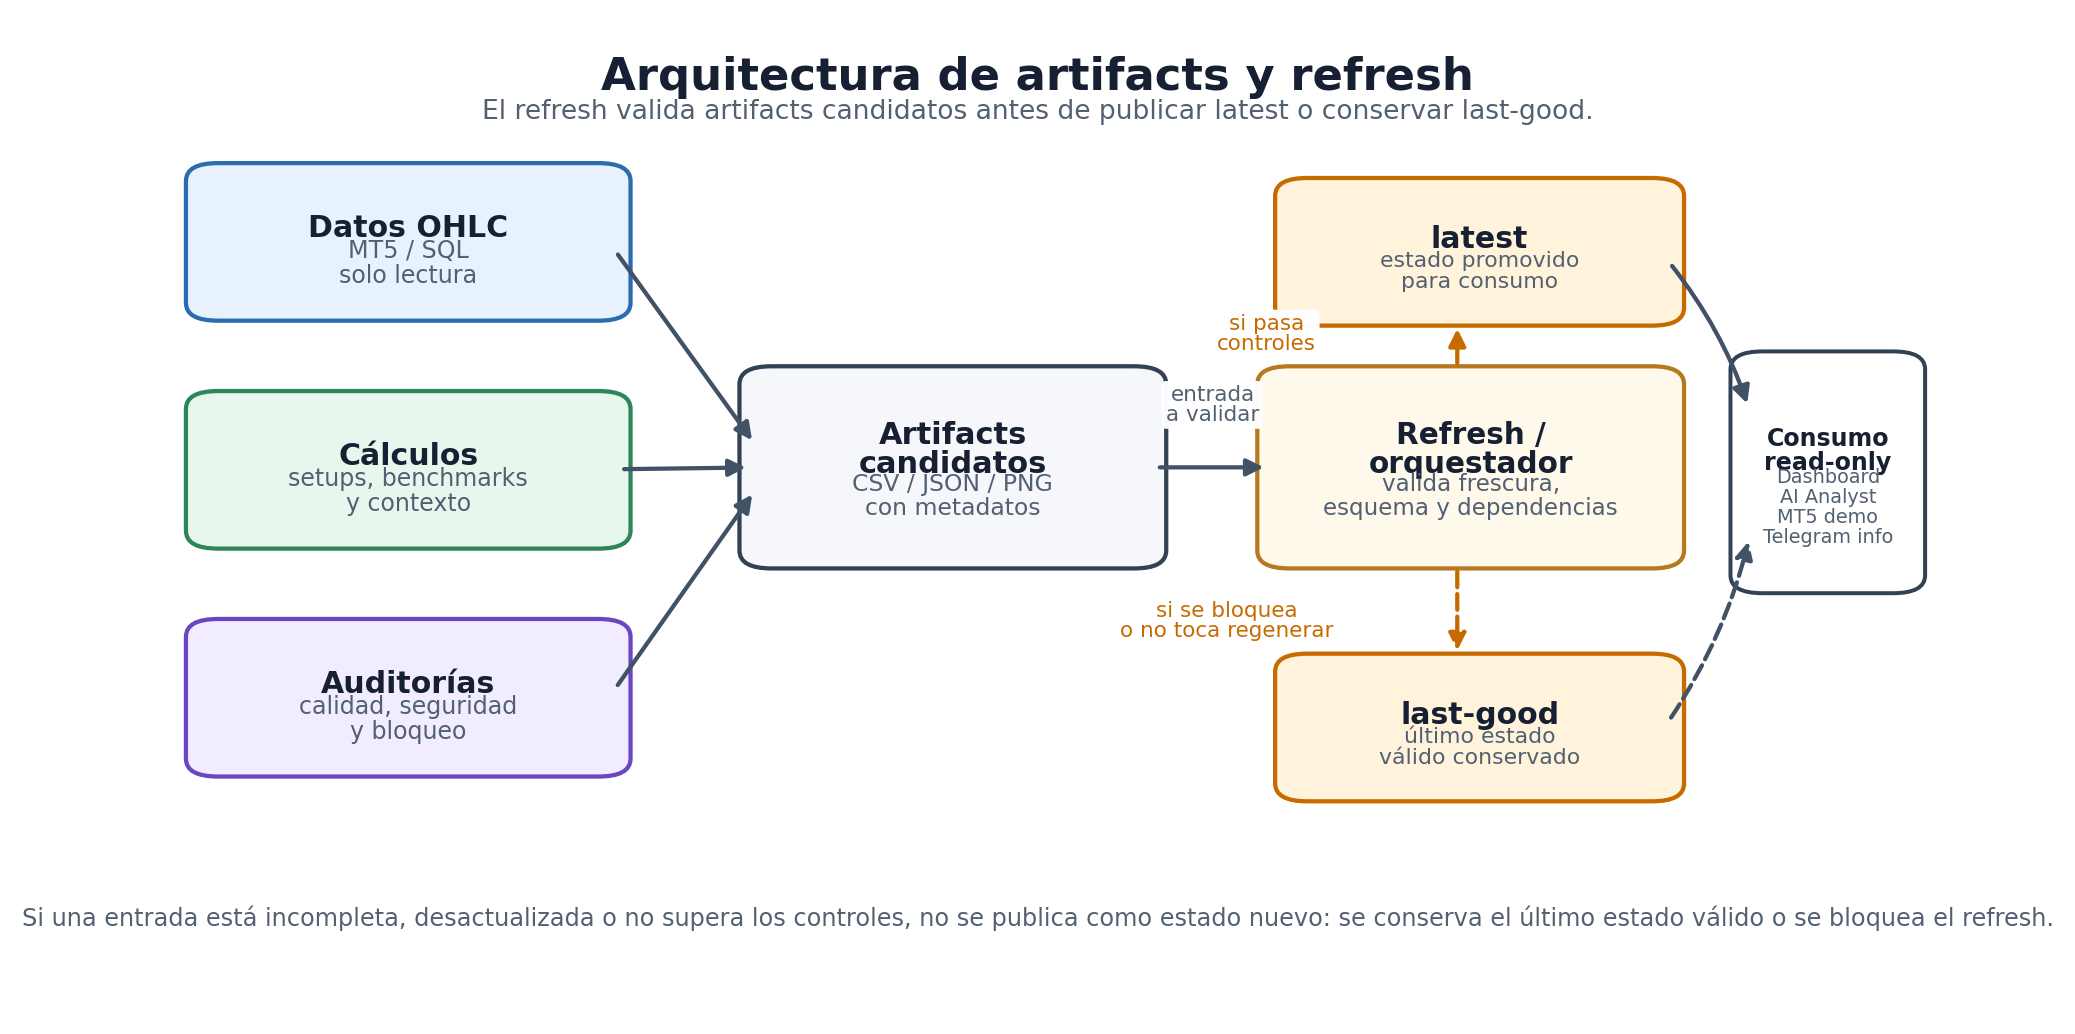
\includegraphics[width=0.98\textwidth]{figs/canonicas/metodologia/arquitectura_artifacts_refresh_canonico.png}
\caption[Arquitectura de archivos de evidencia y actualizaci\'on]{Esquema metodol\'ogico de la arquitectura de archivos de evidencia y
actualizaci\'on. El orquestador valida salidas candidatas antes de publicar un nuevo
estado en \texttt{latest} o conservar \texttt{last-good}; la figura no representa
operaci\'on real ni automatizaci\'on aut\'onoma.}
\label{fig:arquitectura-artifacts-refresh}
\end{figure}

\subsection{Rutas latest y consumo por componentes}
\label{subsec:latest-consumo-componentes}

Para que la plataforma pueda consumir los resultados sin depender de carpetas
fechadas concretas, se introduce una ruta estable de trabajo:
\texttt{trading\_center\_latest}. Esta carpeta act\'ua como punto de entrada para
el dashboard y para otros m\'odulos que necesitan leer el \'ultimo corte v\'alido
de datos. En lugar de buscar manualmente la ejecuci\'on m\'as reciente de cada
fase, los m\'odulos que utilizan esos datos leen una estructura com\'un y un
manifiesto asociado.

El manifiesto \texttt{latest\_manifest.json} cumple una funci\'on de control. No
solo indica que existen archivos disponibles, sino que permite registrar el
momento de publicaci\'on, la decisi\'on del ciclo de actualizaci\'on y los
componentes promovidos. El dashboard utiliza este manifiesto para detectar
cambios y recargar sus datos cuando procede. De esta forma, la interfaz puede
actualizarse al cambiar los archivos publicados sin reiniciar el servidor.

La promoci\'on a \texttt{latest} se realiza por componente. Esto es importante
porque no todas las capas tienen la misma frecuencia natural. Mercado,
contexto Fibonacci o Screener pueden actualizarse en ciclos m\'as r\'apidos,
mientras que correlaciones o WeaveCount pueden mantenerse como \'ultimo resultado
v\'alido si no corresponde recalcularlos en ese ciclo. Esta pol\'itica evita
bloquear toda la plataforma por una capa lenta o por un componente que no ha
producido un corte v\'alido, y al mismo tiempo deja trazabilidad de qu\'e se ha
actualizado y qu\'e se ha conservado.

\subsection{Orquestaci\'on de la actualizaci\'on}
\label{subsec:orquestacion-refresh}

La actualizaci\'on de los archivos publicados se apoya en dos elementos. El
primero es la salida generada por el planificador de datos, que indica
para cada timeframe cu\'al es el cierre
de vela esperado y cu\'al es la \'ultima vela cerrada disponible. Esta indicaci\'on
es necesaria porque el sistema trabaja con velas cerradas y no debe tratar una
vela abierta como dato definitivo. Tambi\'en permite gestionar casos pr\'acticos,
como diferencias horarias del broker o retrasos en timeframes superiores.

El segundo elemento es el orquestador de archivos de evidencia. Su funci\'on es
decidir si una
actualizaci\'on puede ejecutarse, si debe hacerse con advertencias, si debe
bloquearse o si conviene utilizar el \'ultimo conjunto v\'alido de archivos. Esta
decisi\'on se apoya en validaciones de actualidad, disponibilidad y seguridad.
Cuando un componente pasa los controles, puede promoverse a \texttt{latest};
cuando no los pasa, el sistema conserva la salida anterior si sigue siendo
v\'alida para la revisi\'on.

Sobre esa base se implementa un servicio local de actualizaci\'on que coordina el
proceso en modo manual o guiado por la informaci\'on del planificador. El
servicio puede llamar al
orquestador, comparar el manifiesto antes y despu\'es del ciclo, y dejar una
auditor\'ia del cambio producido. Este servicio sirve para validar que el Trading
Center puede actualizar sus datos publicados y que el dashboard puede recoger el
nuevo manifiesto sin reiniciar el servidor. Se considera una validaci\'on local y
controlada del mecanismo de actualizaci\'on: permite comprobar que el flujo
funciona en el entorno del TFG, pero no equivale a haber mantenido el sistema
desplegado de forma continuada durante d\'ias o semanas.

\subsection{Alcance y l\'imites de la actualizaci\'on}
\label{subsec:alcance-limites-refresh}

La arquitectura de actualizaci\'on mantiene los mismos l\'imites de seguridad que el
resto del TFG. No ingiere datos por su cuenta, no escribe en SQL real, no conecta
MT5, no activa Telegram, no genera se\~nales operativas y no env\'ia \'ordenes. Su
papel es coordinar archivos ya generados o validar si una actualizaci\'on puede
promoverse de forma trazable.

Con este alcance, el trabajo cuenta con una arquitectura basada en archivos de evidencia
que permite ordenar resultados, publicar cortes estables y actualizar la
interfaz de revisi\'on en entorno local. Tambi\'en se ha validado el uso de
manifiestos y pol\'iticas de \textit{last-good} para evitar que datos incompletos
o desactualizados sustituyan sin control a salidas previas.

Esta validaci\'on no pretende cerrar la operaci\'on continua del sistema en
producci\'on. La arquitectura permite dar continuidad al flujo de archivos de evidencia y al
dashboard en entorno local. Para considerarla un servicio permanente har\'ian
falta pruebas prolongadas de estabilidad, supervisi\'on de incidencias,
despliegue del scheduler como servicio y validaci\'on continua de fuentes de
datos. En el alcance de este TFG, esta actualizaci\'on se presenta como una capa
metodol\'ogica y t\'ecnica para dar continuidad a la plataforma, no como una
garant\'ia de funcionamiento permanente ni de operaci\'on continuada.

\section{Trading Center Dashboard}
\label{sec:trading-center-dashboard}

\subsection{Funci\'on de integraci\'on}
\label{subsec:dashboard-funcion-integracion}

El Trading Center Dashboard es la capa principal de visualizaci\'on y consulta
del sistema. Se implementa como aplicaci\'on local con Dash \cite{dash_docs}.
Desde esta interfaz se revisa de forma conjunta la informaci\'on generada por el
resto del sistema. Su funci\'on no es decidir por encima de los m\'odulos ya
descritos, sino reunir en una misma interfaz datos de mercado, contexto
estructural, setups, correlaciones, estado del bot y apoyo anal\'itico. Esto
reduce la dispersi\'on de archivos de evidencia y permite que la revisi\'on de
datos de mercado no dependa de abrir manualmente tablas, gr\'aficos y carpetas
separadas.

Esta decisi\'on responde a una necesidad pr\'actica del trabajo. La evaluaci\'on
hist\'orica y la formalizaci\'on de reglas permiten estudiar el comportamiento de
las estrategias. Para que el sistema sea \'util como herramienta de apoyo,
tambi\'en debe presentar datos, m\'etricas y contexto de forma clara y revisable. El dashboard
act\'ua como puente entre los resultados generados por los m\'odulos internos y
una lectura humana supervisada. As\'i, su valor metodol\'ogico est\'a en
ordenar evidencias, no en sustituir la interpretaci\'on final del usuario.

En relaci\'on con la arquitectura descrita en la secci\'on anterior, el
dashboard consume archivos publicados y rutas \texttt{latest}. No recalcula por
s\'i mismo los resultados principales ni se plantea como origen de las pruebas.
Su papel es mostrar el \'ultimo estado disponible, facilitar la comparaci\'on
entre capas y mantener clara la separaci\'on entre datos, contexto, observaci\'on
y ejecuci\'on.

\subsection{Vistas principales de revisi\'on}
\label{subsec:dashboard-vistas-principales}

La organizaci\'on de la interfaz sigue la misma l\'ogica que el resto de la
metodolog\'ia. Las vistas de Mercado y Correlaci\'on proporcionan una primera
lectura del entorno: tendencia, volatilidad, comportamiento relativo de los
activos y relaciones que pueden concentrar riesgo pese a parecer diversificadas.
Estas vistas no generan setups, pero ayudan a interpretar si un posible
candidato aparece en un contexto favorable, ambiguo o excesivamente
correlacionado con otros activos.

La vista WeaveCount incorpora la lectura estructural descrita previamente. En
ella se presentan hip\'otesis de ondas, direcci\'on, timeframe y calidad
visual para que el usuario pueda revisar casos relevantes sin tratarlos como
se\~nales cerradas. Esta informaci\'on se utiliza como contexto estructural de
estudio, especialmente cuando un setup del Screener coincide con una zona o
fase del precio que merece una revisi\'on m\'as detallada.

El Screener funciona como m\'odulo de priorizaci\'on de casos de estudio. Muestra setups principales
como \texttt{macd\_breakout}, \texttt{fib\_limit\_live\_candidate} y
\texttt{rsi\_trend\_reversal}. Adem\'as, los acompa\~na de informaci\'on contextual. La
calidad visual ayuda a priorizar la revisi\'on, pero no representa probabilidad
de acierto ni rentabilidad esperada. De esta forma, el dashboard puede se\~nalar
qu\'e gr\'aficos conviene mirar antes, sin convertir esa priorizaci\'on en una
orden ni en una recomendaci\'on autom\'atica.

El dashboard se completa con el panel MT5 Bot y el AI Analyst. El primero
muestra el estado del proceso asociado al bot, las decisiones auditadas, los
bloqueos de RiskGuard y la informaci\'on de Telegram cuando procede. El segundo
prepara paquetes de revisi\'on y puede generar informes a partir de datos
estructurados y gr\'aficos. Ambos bloques se integran como apoyo a la supervisi\'on
y al an\'alisis, no como mecanismos que autoricen por s\'i mismos una operaci\'on.

\subsection{Revisi\'on visual y trazabilidad}
\label{subsec:dashboard-revision-visual-trazabilidad}

Una parte importante del dashboard es la revisi\'on gr\'afica. En lugar de
limitarse a mostrar una tabla de resultados, la plataforma permite abrir modales
con velas, indicadores y capas de contexto. En el Screener, por ejemplo, el
usuario puede revisar el precio junto a niveles de Fibonacci, pivotes, niveles
redondos, RSI, MACD, tendencia por timeframe y referencias estructurales
cuando est\'an disponibles. Esta visualizaci\'on ayuda a comprobar si el caso
detectado resulta coherente en el gr\'afico antes de pasar a una interpretaci\'on
m\'as profunda.

El uso de modales tambi\'en permite evitar una pantalla principal demasiado
densa. La vista general prioriza los casos y resume el contexto; la vista
detallada conserva las capas necesarias para revisar un activo concreto. Esta
separaci\'on resulta importante porque una herramienta de apoyo al trading puede
perder utilidad si presenta demasiada informaci\'on al mismo tiempo. La
metodolog\'ia seguida busca que el dashboard act\'ue como una mesa de revisi\'on:
primero orienta la atenci\'on y despu\'es permite profundizar en el gr\'afico.

La trazabilidad se mantiene porque cada vista se alimenta de archivos de evidencia
identificables. Un setup mostrado en el Screener, una hip\'otesis de WeaveCount o
un resumen del panel MT5 Bot pueden relacionarse con archivos generados durante
el proceso. Esta relaci\'on evita que la interfaz sea una pantalla opaca: lo que
se muestra procede de salidas auditables y puede contrastarse con las tablas,
informes o registros correspondientes.

\subsection{Separaci\'on entre revisi\'on y ejecuci\'on}
\label{subsec:dashboard-separacion-revision-ejecucion}

El sistema no ejecuta autom\'aticamente cada setup mostrado. La identificaci\'on de un
caso, la validaci\'on de riesgo y el env\'io de \'ordenes se separan en capas
distintas. El dashboard permite revisar el estado de ese proceso, pero cualquier
env\'io queda limitado a un entorno demo controlado y requiere condiciones
expl\'icitas de activaci\'on. La operaci\'on real aut\'onoma queda fuera del alcance del
trabajo.

Esta separaci\'on evita que la interfaz se confunda con una consola operativa.
El dashboard no se utiliza para lanzar \'ordenes desde una vista gr\'afica ni para
confirmar operaciones mediante Telegram. Cuando muestra informaci\'on del bot
MT5, lo hace como seguimiento y auditor\'ia del ciclo controlado. Cuando aparece
Telegram, su papel es informar del estado o de eventos relevantes. Y cuando se
prepara un an\'alisis con AI Analyst, el objetivo es generar una revisi\'on
documentada, no delegar una decisi\'on de entrada o salida.

Con este alcance, el Trading Center Dashboard se entiende como la capa visible de
revisi\'on del sistema. Integra evidencias, facilita la supervisi\'on humana y
ayuda a aprovechar mejor la informaci\'on disponible, pero mantiene separadas las
funciones de estudio, validaci\'on de riesgo y ejecuci\'on. Esta separaci\'on es
necesaria para que el TFG pueda mostrar una plataforma funcional sin afirmar
que se ha desarrollado un sistema de trading real aut\'onomo.

\section{Capa demo controlada: MT5 Bot, RiskGuard y Telegram informativo}
\label{sec:capa-demo-mt5-riskguard-telegram}

\subsection{De lectura MT5 a demostraci\'on controlada}
\label{subsec:mt5-lectura-demostracion-controlada}

La conexi\'on con MetaTrader 5 se introduce en el TFG de forma gradual. El primer
uso es de solo lectura: consultar informaci\'on de cuenta, posiciones, \'ordenes y
s\'imbolos disponibles para incorporarla como evidencia del estado operativo de
la cuenta.
Esta fase permite observar la cuenta y contrastar capturas de estado sin que el
sistema pueda modificar posiciones ni enviar \'ordenes.

Sobre esa base se a\~nade una fase de observaci\'on sin ejecuci\'on. En ella, el
sistema registra qu\'e decisiones podr\'ian haberse planteado a partir de algunos
setups seleccionados, pero sin ejecutar ninguna acci\'on. Esta capa sirve para
separar la detecci\'on de un caso de estudio de cualquier paso posterior. Una
lectura del Screener no pasa directamente a mercado: primero se convierte, si
procede, en una intenci\'on de orden demo, entendida como una propuesta
intermedia que todav\'ia debe ser validada.

La demostraci\'on controlada aparece al final de esa cadena. El objetivo no es
probar un bot preparado para operar con dinero real, sino comprobar que existe
un flujo auditado entre un caso candidato, una validaci\'on de riesgo, un env\'io
demo y una gesti\'on posterior de la posici\'on. Este flujo se plantea como prueba
de integraci\'on entre componentes, siempre dentro de una cuenta demo y bajo
condiciones expl\'icitas de activaci\'on.

\subsection{RiskGuard demo como control previo de riesgo}
\label{subsec:riskguard-limite-riesgo}

RiskGuard se utiliza como capa de control antes de cualquier env\'io demo. Su
funci\'on no es decidir si una estrategia es buena ni mejorar una se\~nal t\'ecnica,
sino comprobar si una posible operaci\'on contiene la informaci\'on m\'inima para
avanzar dentro del flujo demo. Por eso revisa elementos como precio de entrada,
volumen, patrimonio de la cuenta y datos del instrumento. Tambi\'en comprueba el
stop loss, entendido como nivel de salida por p\'erdida m\'axima, y el take profit,
entendido como nivel de salida por beneficio objetivo.

El dimensionamiento del volumen se basa en una cantidad monetaria de riesgo y
en la distancia hasta el stop loss. Si el stop no es v\'alido, si faltan metadatos
relevantes del instrumento o si el riesgo no puede calcularse de forma razonable,
la decisi\'on se bloquea. Esta regla es importante porque evita completar con
suposiciones una informaci\'on que afectar\'ia directamente al tama\~no de la
operaci\'on. En este punto se prioriza la prudencia: ante una entrada ambigua, la
respuesta adecuada del sistema es no avanzar.

Adem\'as del dimensionamiento individual, RiskGuard revisa la exposici\'on
acumulada. Tambi\'en comprueba si existen duplicados, posiciones u \'ordenes
incompatibles, l\'imites por s\'imbolo, l\'imite total y, cuando la informaci\'on lo
permite, exposici\'on por grupo de activos. Se incorpora adem\'as un estado de
bloqueo por p\'erdida diaria o acumulada en demo. Estas comprobaciones no
convierten la capa en un control suficiente para operar en una cuenta real, pero
s\'i permiten describirla como una capa demo m\'as robusta y auditable dentro del
alcance acad\'emico del trabajo.

\subsection{Env\'io y gesti\'on de \'ordenes demo}
\label{subsec:envio-gestion-ordenes-demo}

El m\'odulo de env\'io demo solo interviene despu\'es de que exista una propuesta
aceptada por RiskGuard y se cumplan las condiciones expl\'icitas configuradas
para la prueba. No toma decisiones directamente desde el Screener ni transforma
cualquier setup mostrado en una orden. La separaci\'on entre identificaci\'on,
validaci\'on y env\'io permite revisar cada paso de forma independiente y dejar
registro de por qu\'e una operaci\'on demo se acepta o se bloquea.

La gesti\'on posterior de posiciones demo sigue la misma l\'ogica. El cierre no se
plantea como una acci\'on autom\'atica general sobre cualquier posici\'on abierta,
sino como una actuaci\'on controlada sobre una posici\'on identificada y
auditada. Esta precauci\'on evita decisiones ambiguas, especialmente en
escenarios donde podr\'ian existir varias posiciones del mismo activo o estados
intermedios no previstos.

La validaci\'on realizada debe interpretarse como demostraci\'on de una cadena
t\'ecnica completa en demo. Se comprueba que los componentes pueden comunicarse,
que las decisiones quedan registradas y que una posici\'on demo puede enviarse y
cerrarse dentro del flujo previsto. Sin embargo, esta evidencia no equivale a
una validaci\'on de operaci\'on continua. Tampoco permite afirmar que el sistema
est\'e preparado para operar en una cuenta real sin nuevas pruebas, supervisi\'on
y controles adicionales.

\subsection{Telegram como canal informativo}
\label{subsec:telegram-observabilidad-informativa}

Telegram se incorpora como canal de informaci\'on del MT5 Bot. Su papel es
notificar o resumir eventos relevantes del sistema: estado del bot, lectura de
cuenta, posiciones abiertas, \'ordenes demo auditadas, cierres demo, bloqueos de
RiskGuard, errores de actualizaci\'on y res\'umenes de seguimiento. Esta capa
busca que el usuario pueda recibir informaci\'on compacta sin abrir
necesariamente el dashboard \cite{telegram_bot_api}.

La funci\'on de Telegram se mantiene separada de la ejecuci\'on. Los mensajes no
solicitan confirmaciones, no reciben comandos y no permiten abrir, cerrar o
modificar operaciones. Esta decisi\'on evita convertir un canal de notificaci\'on
en una consola de trading, lo que introducir\'ia riesgos de seguridad y de
interpretaci\'on fuera del objetivo del TFG.

En la metodolog\'ia del trabajo, Telegram se entiende como un mecanismo de
seguimiento. Ayuda a comunicar el estado del sistema y a dejar constancia de
eventos relevantes, pero no participa en la decisi\'on operativa. Por ello,
aunque se haya validado el formato de mensajes informativos, su alcance final
queda limitado a seguimiento y notificaci\'on.

\subsection{Alcance final de la capa demo}
\label{subsec:alcance-final-capa-demo}

En conjunto, esta capa permite comprobar que el sistema puede pasar de una
se\~nal de estudio a una operaci\'on demo auditada manteniendo separadas la
detecci\'on, el control de riesgo, la ejecuci\'on controlada y la comunicaci\'on
informativa. Esta separaci\'on es esencial para que el trabajo pueda mostrar una
integraci\'on funcional sin confundirla con un sistema de operaci\'on con dinero
real.

Lo que queda cerrado para la memoria es una cadena demo controlada y trazable.
MT5 aporta lectura y ejecuci\'on demo bajo condiciones expl\'icitas, RiskGuard
act\'ua como control previo de riesgo y Telegram informa sobre el estado del
proceso. Cada componente tiene una funci\'on concreta y ninguno de ellos elimina la
necesidad de supervisi\'on humana.

La operaci\'on real, la autonom\'ia continua, la validaci\'on prolongada y el uso
de Telegram como mecanismo de control quedan fuera del alcance del TFG. Esta
limitaci\'on no invalida la aportaci\'on de la capa demo; al contrario, delimita
con precisi\'on qu\'e se ha demostrado y qu\'e requerir\'ia una fase posterior de
desarrollo y evaluaci\'on.

\section{AI Analyst como asistente de revisi\'on de solo lectura}
\label{sec:ai-analyst-read-only}

\subsection{Papel dentro del sistema}
\label{subsec:ai-analyst-papel-sistema}

El AI Analyst se incorpora como una capa de apoyo a la revisi\'on humana. Su
funci\'on se sit\'ua al final del flujo de revisi\'on, cuando el sistema ya dispone
de informaci\'on suficiente para analizar un caso concreto. Esa informaci\'on puede incluir
setups del Screener, contexto de mercado, correlaciones, hip\'otesis de
WeaveCount o gr\'aficos asociados. En lugar de
obligar al usuario a revisar todos esos elementos de forma aislada, el asistente
ayuda a organizarlos y a convertirlos en una lectura documentada.

Esta capa no se plantea como un modelo que decida operaciones. Su valor est\'a en
resumir informaci\'on, se\~nalar puntos de atenci\'on, relacionar contexto y generar
un informe que pueda revisarse posteriormente. La decisi\'on final sigue
perteneciendo al usuario y a las capas de control definidas en el trabajo. Por
ello, AI Analyst no sustituye al criterio del usuario, no aprueba entradas y no
reemplaza a RiskGuard.

Dentro de la metodolog\'ia, AI Analyst conecta datos, gr\'afico e interpretaci\'on
textual. El dashboard permite localizar el caso, los archivos de evidencia
conservan el material utilizado y el asistente genera una revisi\'on estructurada.
Esta revisi\'on puede incluirse como informe o anexo. De esta forma, la revisi\'on asistida queda integrada en el
sistema sin convertirse en una capa operativa aut\'onoma.

\subsection{Paquetes trazables de revisi\'on}
\label{subsec:ai-analyst-paquetes-reproducibles}

Antes de generar un an\'alisis, el sistema prepara un paquete de revisi\'on. Este
paquete contiene la informaci\'on necesaria para interpretar el caso: datos
estructurados, gr\'afico asociado, tipo de an\'alisis solicitado y referencias a
las fuentes locales utilizadas. El an\'alisis no se realiza, por tanto, a partir
de una pregunta libre ni de una captura aislada, sino a partir de un conjunto de
informaci\'on organizado y trazable.

Con ello se reduce la ambig\"uedad del an\'alisis. Un comentario generado solo a
partir de una imagen podr\'ia omitir el origen de los datos, el contexto del
setup o el timeframe de la revisi\'on. Al preparar un paquete, el asistente
recibe una versi\'on ordenada del caso y el usuario puede comprobar despu\'es qu\'e
informaci\'on se utiliz\'o para construir el informe.

Sobre ese material preparado, la revisi\'on puede lanzarse de forma expl\'icita
desde el entorno local mediante Codex CLI \cite{openai_codex_cli_docs}. En este caso, Codex CLI act\'ua como
asistente de an\'alisis del contexto reunido por el sistema, no como un componente
conectado a MT5 ni a una capa operativa. Por ello, la integraci\'on mantiene el
car\'acter de solo lectura del AI Analyst.

Los paquetes pueden corresponder a distintos tipos de revisi\'on. En un setup del
Screener se incluyen las reglas principales, el contexto y el gr\'afico. En una
hip\'otesis de WeaveCount se incorporan los puntos estructurales y la lectura de
onda. En una correlaci\'on se preparan las m\'etricas y el gr\'afico del par
seleccionado. Esta organizaci\'on permite que AI Analyst mantenga el foco del
an\'alisis y no mezcle elementos que pertenecen a capas distintas.

\subsection{Informes y contexto externo}
\label{subsec:ai-analyst-informes-contexto}

El resultado principal del AI Analyst es un informe de revisi\'on. Este documento
resume el caso, presenta los datos utilizados, incorpora el gr\'afico cuando
procede y expone una interpretaci\'on razonada. El formato resulta \'util para
documentar por qu\'e un caso puede ser interesante, qu\'e cautelas presenta y qu\'e
elementos de contexto conviene revisar antes de tomar una decisi\'on supervisada.

El asistente tambi\'en puede incorporar contexto externo cuando se solicita de
forma expl\'icita. Esta opci\'on se reserva para situaciones en las que noticias,
calendario macroecon\'omico o informaci\'on institucional puedan afectar a la
lectura del mercado. En el TFG, este contexto se trata de forma separada de los
datos de mercado estructurados, ya que su disponibilidad, coste o forma de
acceso puede variar.

Por este motivo, la informaci\'on externa no se utiliza como si fuera una tabla
hist\'orica m\'as del sistema. Cuando se incorpora, debe entenderse como apoyo
interpretativo y no como base cuantitativa del backtesting. Si el asistente no
puede verificar una fuente o el contexto no es concluyente, la salida debe
reflejar esa incertidumbre en lugar de transformarla en una conclusi\'on
operativa.

\subsection{L\'imites de decisi\'on y seguridad}
\label{subsec:ai-analyst-limites-decision-seguridad}

La respuesta del AI Analyst se interpreta como una revisi\'on documentada. Puede
aportar argumentos, advertencias o contexto adicional, pero no valida una
operaci\'on ni desbloquea la ejecuci\'on. El asistente no conecta con MT5, no env\'ia
\'ordenes, no activa Telegram de forma autom\'atica y no escribe resultados
operativos en la base de datos.

Esta separaci\'on es necesaria porque un modelo de lenguaje puede ayudar a ordenar
informaci\'on, pero no debe confundirse con una validaci\'on de riesgo ni con una
autorizaci\'on operativa. Aunque el informe pueda resultar \'util para entender un
caso, la validaci\'on de riesgo y cualquier paso relacionado con ejecuci\'on demo
pertenecen a capas separadas. Si una salida no cumple el formato esperado o no
puede generarse con garant\'ias suficientes, el sistema debe dejar constancia del
problema y remitir la revisi\'on al usuario.

As\'i, AI Analyst se mantiene como una herramienta de apoyo. Su incorporaci\'on
mejora la capacidad de revisar casos complejos y documentar razonamientos. No
altera el alcance del TFG: la plataforma sigue siendo una base de an\'alisis,
validaci\'on y demostraci\'on controlada, no un sistema que delegue decisiones
operativas en un modelo generativo.

Como evidencia documental, esta capa se apoya en capturas del panel y en un
informe PDF incluido en anexos. No se presenta como sustituto de los resultados
cuantitativos, sino como ejemplo de revisi\'on asistida: datos utilizados,
gr\'afico, contexto, interpretaci\'on y cautelas. Esta distinci\'on permite
presentar el AI Analyst como parte del flujo de an\'alisis sin sobreafirmar su
papel.
